% Template for a Computer Science Tripos Part II project dissertation
\documentclass[12pt,a4paper,twoside,openright]{report}
\usepackage[hyphens]{url}
\usepackage[pdfborder={0 0 0}]{hyperref}    % turns references into hyperlinks
\usepackage[nameinlink]{cleveref}
\crefname{algorithm}{Algorithm}{Algorithms}
\crefname{figure}{Figure}{Figures}
\crefname{listing}{Listing}{Listings}
\crefname{section}{Section}{Sections}


\usepackage[margin=25mm]{geometry}  % adjusts page layout
\usepackage{graphicx}  % allows inclusion of PDF, PNG and JPG images
\usepackage{verbatim}
\usepackage{docmute}   % only needed to allow inclusion of proposal.tex
\usepackage{todonotes}
\usepackage{algpseudocode}
\usepackage{algorithm}
\usepackage{tabularx}
\usepackage[numbers]{natbib}
\usepackage{tikz}
\usepackage{caption}
\usepackage{subcaption}
\captionsetup[figure]{labelfont={bf},textfont=it}
\usetikzlibrary{trees,calc,matrix,arrows,decorations.pathreplacing}
\usepackage{gnuplot-lua-tikz}

\tikzset{>=stealth'}

%%%%%%% Using Minted Package for Code Listings %%%%%%%
\usepackage{minted}
\usemintedstyle{colorful}

\raggedbottom                           % try to avoid widows and orphans
\sloppy
\clubpenalty1000%
\widowpenalty1000%

\renewcommand{\baselinestretch}{1.1}    % adjust line spacing to make
                                        % more readable

\newcommand{\mytodo}{\todo[inline, color=green!40]}

\begin{document}

\bibliographystyle{plainnat}

%%%%%%%%%%%%%%%%%%%%%%%%%%%%%%%%%%%%%%%%%%%%%%%%%%%%%%%%%%%%%%%%%%%%%%%%
% Title


\pagestyle{empty}

\rightline{\LARGE \textbf{Rupert Horlick}}

\vspace*{60mm}
\begin{center}
\Huge
\textbf{Encrypted Keyword Search Using Path ORAM on MirageOS} \\[5mm]
Computer Science Tripos -- Part II \\[5mm]
Homerton College \\[5mm]
\today  % today's date
\end{center}

%%%%%%%%%%%%%%%%%%%%%%%%%%%%%%%%%%%%%%%%%%%%%%%%%%%%%%%%%%%%%%%%%%%%%%%%%%%%%%
% Proforma, table of contents and list of figures

\pagestyle{plain}

\chapter*{Proforma}

{\large
\begin{tabular}{ll}
Name:               & \bf Rupert Horlick                       \\
College:            & \bf Homerton College                     \\
Project Title:      & \bf Encrypted Keyword Search Using \\
& \bf Path ORAM on MirageOS \\
Examination:        & \bf Computer Science Tripos -- Part II, July 2016  \\
Word Count:         & \bf \footnotemark[1]
                      (well less than the 12000 limit)  \\
Project Originator: & Dr Nik Sultana                    \\
Supervisors:         & Dr Nik Sultana \& Dr Richard Mortier                    \\
\end{tabular}
}
\footnotetext[1]{This word count was computed
by \texttt{detex diss.tex | tr -cd '0-9A-Za-z $\tt\backslash$n' | wc -w}
}
\stepcounter{footnote}


\section*{Original Aims of the Project}

% Give a 100 word summary of what was to be achieved by the project, i.e. secure searchable encrypted documents

\section*{Work Completed}



\section*{Special Difficulties}



\newpage
\section*{Declaration}

I, Rupert Horlick of Homerton College, being a candidate for Part II of the Computer
Science Tripos, hereby declare
that this dissertation and the work described in it are my own work,
unaided except as may be specified below, and that the dissertation
does not contain material that has already been used to any substantial
extent for a comparable purpose.

\bigskip
\leftline{Signed [signature]}

\medskip
\leftline{Date [date]}

\tableofcontents

\listoffigures

%\todototoc
%\listoftodos

%%%%%%%%%%%%%%%%%%%%%%%%%%%%%%%%%%%%%%%%%%%%%%%%%%%%%%%%%%%%%%%%%%%%%%%
% now for the chapters

\pagestyle{headings}

\chapter{Introduction}

\section{Motivation}

With cloud storage fast becoming ubiquitous, providers are faced with the challenge of guaranteeing the security of their clients' data. 
More than an exabyte of data was delivered by cloud storage providers in 2013 \cite{nasuni2013cloud}, and since so much of this data is held by only a handful of providers, trust is becoming a major concern.

Encryption might appear to be the solution to these trust issues; surely if the providers cannot read the plain-text of data then it must be secure. This seems to hold in general, but, in the application of query-based search, there is a problem. \citet{islam2012access} demonstrated that using current methods of homomorphic encryption to search over encrypted documents can leak up to 80\% of queries. Knowledge of the queries made to a data set, along with the number of documents returned by each query, could lead to dangerous inferences. As a motivating example, the discovery that a query to a medical database, such as $\langle name,~disease\rangle$, returned results might allow an adversary to deduce information about a patient's medical status, constituting a breach of patient confidentiality.

\citet{islam2012access} were able to infer search queries using the access pattern, the set of documents returned by each query. Thus, in order to protect against this kind of attack, we need to prevent the server from knowing which documents it returns in response to a query. Oblivious Random-Access Memory (ORAM) provides exactly that. Using ORAM, two accesses to the same piece of data, and, moreover, any two access patterns of the same length, are computationally indistinguishable to the server.

This project aims to demonstrate that, using \citeauthor{stefanov2013path}'s Path ORAM protocol \cite{stefanov2013path}, it is possible to build a system that searches over encrypted documents without leaking the resulting access pattern, protecting the content of the search queries and, therefore, the confidentiality of the documents.

\section{Challenges}

When dealing with security, the first challenge is to precisely define the threat model. The assumed capabilities of all parties must be clearly stated to ensure that security proofs are built on a solid foundation. The threat model for this project was refined a number of times, following the discovery of hidden assumptions, and is defined in \cref{sec:threatmodel}.

Another challenge is taking a complex, abstract protocol, and making the design decisions required to turn it into a working system. The Path ORAM protocol abstracts away many implementation details, which had to be realised in this project.

Adding recursion to ORAM reduces the amount of client-side storage, making stateless ORAM more efficient. This presents us with the challenge of building recursive data structures, which are difficult to reason about and debug. This project takes advantage of OCaml's powerful module system, which separates the challenge of recursion from the underlying implementation.

The final challenge is choosing how to evaluate ORAM. There are many parameters and metrics that we could examine, however, due to the time consuming nature of running experiments on ORAM, this project limits its focus to the time overheads incurred by ORAM and the security of its construction.

\section{Related Work}

ORAM was first introduced by \citet{goldreich1996software} in \citeyear{goldreich1996software}, who were motivated by the need for software protection on disks. The model was then expanded and refined for other settings, such as secure processors and cloud computing \cite{shi2011oblivious}. \citet{stefanov2013path} made a significant contribution to the field, due to the simplicity and elegance of their protocol. Since then, many optimisations and additional features have been developed \cite{yu2014enhancing,ren2015constants,moataz2015resizable}, and used to build a working, cloud-based storage system \cite{stefanov2013oblivistore}. A useful thesis by \citet{teeuwen2015evolution} summarises the entire ORAM field, providing valuable insight into the evolution of ORAM.

\chapter{Preparation}

\section{Threat Model}
\label{sec:threatmodel}

This threat model involves three principals: the client, the server, and the attacker. The network is assumed to be under the control of the attacker. The attacker and the server are defined to be passive, and honest, but curious; they will both gather as much information as possible, without deviating from the protocol. Thus, the attacker will eavesdrop, but will neither prevent transmissions between the client and the server, nor tamper with, or produce their own, messages. The server will not tamper with the underlying storage. In this model, the attacker can be dealt with by the use of encryption, so it is the server that presents a threat, because it can see the access pattern of the underlying storage. The goal of this project is to ensure that this access pattern does not leak information from the search queries nor from the documents in the underlying storage.

%\setlength{\unitlength}{0.67mm}
%\begin{figure}
\begin{center}
\begin{picture}(170,75)
\put(0,0){\framebox(50,30){Client}}

\put(50,15){\vector(1,0){70}}
\put(120,15){\vector(-1,0){70}}

\put(120,0){\framebox(50,30){Server}}

\put(60,45){\framebox(50,30){Attacker}}

\put(85,15){\vector(0,1){30}}
\put(58,7){Read, Write, Search}

\end{picture}
\end{center}
\caption{The Threat Model: The Attacker and Server are honest, but curious}
\label{threatmodel}
\end{figure}
%\setlength{\unitlength}{0.5mm}

\begin{figure}
    \centering
    \begin{tikzpicture}[>=stealth']
        \matrix (m) [matrix of nodes,row sep=8mm,column sep=5mm,nodes={minimum width=35mm,minimum height=20mm,inner sep=0}] {
          &
          |[draw]| Attacker &
          \\
          |[draw]| Client &
          |[minimum size=0]| &
          |[draw]| Server \\
        };
        \draw[->] ($(m-2-2) + (0,1.5mm)$) -- (m-1-2);
        \draw[<->] (m-2-1) -- (m-2-3);
        \node at ($(m-1-2) - (0,34mm)$) {Read, Write, Search};
    \end{tikzpicture}
    \caption{The threat model: the attacker and server are passive, and honest, but curious.}
    \label{fig:threatmodel}
\end{figure}

\section{Introduction to Path ORAM}
\label{sec:oramintro}

The Path ORAM protocol is defined in terms of a client and a server, where the client stores data on the server. The data is divided into \emph{blocks}, each of which is tagged with its offset in the data. We call this the block's \emph{address}.

On the server, blocks are stored in a binary tree of height $L$. Each node in the tree is a \emph{bucket} of size $Z$, that may hold up to $Z$ real blocks. Buckets must always be full, so dummy blocks are stored when there are fewer than $Z$ real blocks. Thus, the tree stores $$N = Z \cdot (2^{L+1} - 1)$$ blocks in total.

The client stores two local data structures: the \emph{stash} and the \emph{position map}. The stash is a sort of working memory. As blocks are read from the server, they are written into the stash and may be returned to the server later on. Initially the stash is empty. The \emph{position map} associates each address with a position between $0$ and $2^L-1$, which corresponds to a leaf, and therefore a path, in the tree. The position map is initialised by assigning a random position to each address.

The protocol maintains the invariant that, after the client performs a read or a write, a block with position $x$ is either in the stash, or in some bucket along the path to leaf $x$. This is achieved by using \cref{alg:access} for both read and write operations. Its execution can be divided into four steps:

\begin{enumerate}
	\item \textbf{Remap block}. The current position $x$ of the block with address $\mathsf{a}$ is read from the position map. A new position is chosen uniformly at random from $\{0,\dots,2^L-1\}$ and is added to the position map.
	\item \textbf{Read path}. The path to leaf $x$ is read into the stash. The block with address $\mathsf{a}$ will now be in the stash, if it has ever been written into ORAM.
	\item \textbf{Write new data}. If the operation is a $\mathsf{write}$, the current block with address $\mathsf{a}$ is removed from the stash and is replaced by the new block containing $\mathsf{data^\ast}$.
	\item \textbf{Write path}. The path to leaf $x$ is filled with blocks from the stash that meet the following condition. A block with address $\mathsf{a'}$ can be written into the bucket at level $l$ if the path to leaf $\mathsf{position[a']}$ follows the path to leaf $x$ down to level $l$. If the number of blocks that satisfy this criterion is less than the bucket size, then the remainder of the bucket is filled with dummy blocks.
\end{enumerate}

If a block in the stash is written back into the tree, then it must be in some bucket along the path to its assigned position. If not, then it is still in the stash, so the invariant holds after each execution of the algorithm.

\begin{algorithm}[h]
\caption{Read/write data block with address $\mathsf{a}$}
\label{alg:access}
\footnotesize
\begin{algorithmic}[1]
    \vskip 10pt
    \Function{Access}{$\mathsf{op,a,data^*}$}
    \vskip 10pt
    \State $x \gets \mathsf{position[a]}$
    \State $\mathsf{position[a]} \gets$ \Call{UniformRandom}{$2^L-1$}
    \vskip 10pt
    \For{$l \in \{0,1,\dots,L\}$}
    	\State $S \gets S~\cup$ \Call{ReadBucket}{$\mathcal{P}(x,l)$}
    \EndFor
    \vskip 10pt
    \State $\mathsf{data} \gets$ Read block $\mathsf{a}$ from $S$
    \If{$\mathsf{op} = \mathsf{write}$}
    	\State $S \gets (S - \{(\mathsf{a,data})\}) \cup \{(\mathsf{a,data^*})\}$
    \EndIf
    \vskip 10pt
    \For{$l \in \{L,L-1,\dots,0\}$}
    	\State $S' \gets \{(\mathsf{a',data'}) \in S : \mathcal{P}(x,l) = \mathcal{P}(\mathsf{position[a']},l)\}$
    	\State $S' \gets$ Select $\min(|S'|,Z)$ blocks from $S'$
    	\State $S \gets S - S'$
    	\State \Call{WriteBucket}{$\mathcal{P}(x,l),S'$}
    \EndFor
    \vskip 10pt
    \State \Return $\mathsf{data}$
    \vskip 10pt
    \EndFunction
    \vskip 10pt
\end{algorithmic}
\end{algorithm}

The security of this algorithm is based on the random assignment of positions in step 1. If we consider the sequence of $M$ accesses, $$\mathbf{p} = (\mathsf{position}_M[\mathsf{a}_M], \mathsf{position}_{M-1}[\mathsf{a}_{M-1}], \dots, \mathsf{position}_1[\mathsf{a}_1]),$$ any two accesses to the same address will be statistically independent, as will two accesses to different addresses. Thus, by an application of Bayes' rule, we have $$\Pr(\mathbf{p}) = \prod\limits^{M}_{j=1}\Pr(\mathsf{position}_j[\mathsf{a}_j]) = \left(\frac{1}{2^L}\right)^M$$ i.e. the probability of the whole sequence is equal to the product of the individual probabilities, and therefore the access pattern is indistinguishable from a random sequence of bit strings.

To enable the client to disconnect from ORAM and reconnect later on, perhaps from a different machine, there must be no persistent client-side state. We call this \emph{stateless} ORAM. This can be achieved by flushing the state, i.e. the stash and the position map, to disk after every operation. However, in the current model, the stash occupies $O(\log N)$ space, and the position map, $O(N)$, making this infeasible in practice.

\emph{Recursive} ORAM reduces the space required by the position map to $O(1)$, taking the overall client-side state to $O(\log N)$. This means that statelessness no longer increases the asymptotic bandwidth overhead. Recursion stores the position map of the original ORAM, now referred to as ORAM$_0$, in another ORAM, ORAM$_1$. Thus, the client-side state becomes the position map of ORAM$_1$, along with the stashes of both ORAM$_0$ and ORAM$_1$. If each block in ORAM$_1$ can store $\chi$ positions then it will need $N' = N/\chi$ blocks. Therefore, the position map of ORAM$_1$ occupies $O(N/\chi)$ space. Repeating this recursion $\log N / \log \chi$ times leads to a position map of size $O(1)$. This sacrifices the space occupied by the recursive ORAMs and the time needed to perform recursive accesses, for efficient statelessness.

\section{Introduction to Inverted Indexes}
\label{sec:invertedindexintro}

The \emph{inverted index} is the most important data structure in Information Retrieval. The amount of time required to perform a query is reduced by performing a large amount of work in advance. A simple linear scan of $N$ documents takes $O(N)$ time. Using an inverted index also takes $O(N)$ time in the worst case, but the constant is greatly reduced and empirically the index delivers excellent performance.

The index consists of two parts: the \emph{dictionary} and the \emph{postings}. The dictionary is a list, usually stored as a hash table, of all of the terms that appear in a set of documents. Each term has a postings list, a list of all the documents that contain that term. Collectively these postings lists are referred to as the postings.

An inverted index can be constructed in three steps:
\begin{enumerate}
    \item Split each document into \emph{tokens}. These are units of the document separated by spaces.
    \item Perform linguistic preprocessing on the tokens. An example is \emph{stemming}, which removes suffixes of words, converting them into a normalised form.
    \item Assuming each document has an ID, add the ID to the postings list of each token the document contains.
\end{enumerate}

Look-up of a single keyword in a hash-based inverted index is performed by hashing the keyword and returning the relevant postings list, if it exists. Simple Boolean operations can be added. For instance, disjunction takes the union of two postings lists, and conjunction takes the intersection.

This project will limit its focus to conjunctive queries, as it aims to demonstrate the correctness and efficiency of search using the ORAM implementation, rather than creating an advanced IR system. Queries are space-separated lists of keywords, and the result of a query is the conjunction of the postings lists of all keywords it contains.

\begin{figure}
    \centering
    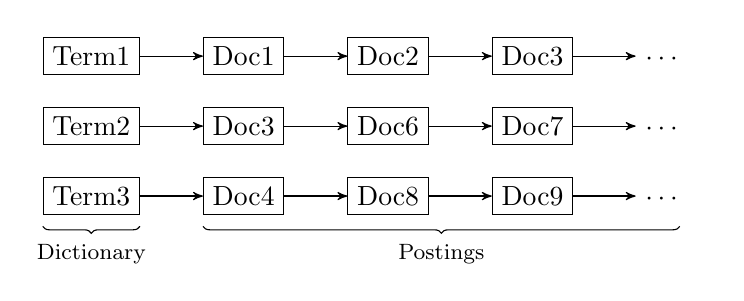
\begin{tikzpicture}
        \matrix (m) [matrix of nodes,nodes={draw},column sep=8mm,row sep=4mm] {
          Term1 & Doc1 & Doc2 & Doc3 & |[draw=none]| $\cdots$\phantom{T} \\
          Term2 & Doc3 & Doc6 & Doc7 & |[draw=none]| $\cdots$\phantom{T} \\
          Term3 & Doc4 & Doc8 & Doc9 & |[draw=none]| $\cdots$\phantom{T} \\
        };
        \draw[->] (m-1-1) -- (m-1-2);
        \draw[->] (m-1-2) -- (m-1-3);
        \draw[->] (m-1-3) -- (m-1-4);
        \draw[->] (m-1-4) -- (m-1-5);
        \draw[->] (m-2-1) -- (m-2-2);
        \draw[->] (m-2-2) -- (m-2-3);
        \draw[->] (m-2-3) -- (m-2-4);
        \draw[->] (m-2-4) -- (m-2-5);
        \draw[->] (m-3-1) -- (m-3-2);
        \draw[->] (m-3-2) -- (m-3-3);
        \draw[->] (m-3-3) -- (m-3-4);
        \draw[->] (m-3-4) -- (m-3-5);
        \draw[decorate,decoration={brace,mirror,raise=4pt}] (m-3-1.south west) -- node[midway,below,yshift=-7pt] {\footnotesize Dictionary} (m-3-1.south east);
        \draw[decorate,decoration={brace,mirror,raise=4pt}] (m-3-2.south west) -- node[midway,below,yshift=-7pt] {\footnotesize Postings} ($(m-3-5.south east) - (1em,0)$);
    \end{tikzpicture}
    \caption{The structure of an inverted index: the dictionary contains terms and the postings contains lists of documents that each term appears in.}
    \label{fig:invertedIndex}
\end{figure}

\section{Introduction to MirageOS}

Running ORAM in the cloud allows a user to access their data from any location. The ORAM client is a trusted cloud instance, and the server is a cloud storage provider, as illustrated in \cref{fig:cloudInstance}.

\begin{figure}
    \centering
    \tikzstyle{principal}=[draw,node distance=50mm,minimum width=30mm,minimum height=25mm,text width=20mm,text centered]
    \begin{tikzpicture}
        \node[principal] (user) {User};
        \node[principal,right of=user] (ci) {Cloud Instance};
        \node[principal,right of=ci] (csp) {Cloud Storage Provider};
        \draw[<->] (user) -- (ci);
        \draw[<->] (ci) -- (csp);
        \draw[decorate,decoration={brace,mirror,raise=4pt}] (ci.south west) -- (csp.south east) node[midway,below,yshift=-4mm] {Path ORAM Protocol};
    \end{tikzpicture}
    \caption{ORAM can be built as a MirageOS application, which can run on a trusted cloud instance.}
    \label{fig:cloudInstance}
\end{figure}

MirageOS is a unikernel operating system. In other words, a MirageOS application is compiled to an executable, along with only the necessary parts of the OS. It can be compiled for a number of targets, including Unix or Xen. An executable, running directly on the Xen hypervisor in the cloud, is more lightweight than the traditional cloud stack, which runs an application on a full operating system, such as Ubuntu. By building ORAM as a MirageOS application, this project allows an instance running ORAM to be spun up whenever the user needs, and shut down when not in use, minimising its cost.

\section{System Architecture}

\setlength{\unitlength}{0.75mm}
\begin{figure}[t]
    \centering
    \begin{picture}(170,70)
        \put(50,60){\framebox(50,10){File system}}
        
        \put(100,65){\vector(1,0){20}}
        \put(120,65){\vector(-1,0){20}}
        
        \put(120,60){\framebox(50,10){Search module}}
        
        \multiput(44,55)(4,0){32}{\line(1,0){2}}
        \put(0,54){\texttt{BLOCK} Interface}
        \put(75,60){\vector(0,-1){10}}
        \put(75,50){\vector(0,1){10}}
        
        %\put(145,45){\vector(0,1){15}}
        %\put(145,45){\vector(-1,0){45}}
        
        \put(50,40){\framebox(50,10){ORAM}}
        
        \multiput(44,35)(4,0){32}{\line(1,0){2}}
        \put(0,34){\texttt{BLOCK} Interface}
        \put(75,40){\vector(0,-1){10}}
        \put(75,30){\vector(0,1){10}}
        
        \put(50,20){\framebox(50,10){Encryption}}
        
        \multiput(44,15)(4,0){32}{\line(1,0){2}}
        \put(0,14){\texttt{BLOCK} Interface}
        \put(75,20){\vector(0,-1){10}}
        \put(75,10){\vector(0,1){10}}
        
        \put(50,0){\framebox(50,10){\texttt{BLOCK}}}
    \end{picture}
    \caption{The application stack: ORAM satisfies MirageOS's \emph{\texttt{BLOCK}} interface and any underlying \emph{\texttt{BLOCK}} implementation can be used.}
    \label{fig:miragestack}
\end{figure}
\setlength{\unitlength}{0.5mm}

We have discussed a couple of the major building blocks of the implementation, but how does it all fit together? We start with the architecture that we already have, a client and a server, communicating using the server's cloud storage API. Now what we want to do is insert our trusted ORAM instance in between the client and the server. In order to do this with the least inconvenience to the user, we need to define an API that unifies those of the cloud providers, providing all of the same facilities that the user already has access to. Then we need to have ORAM actually interface with the cloud providers. We can do this by creating a module for each provider that translates their individual API to satisfy MirageOS's BLOCK interface. Actually writing these modules will not be part of this project.

Now all of the important stuff can happen in between the two interfaces. \Cref{fig:miragestack} shows the overall structure of the ORAM instance. From the bottom up, we have the underlying BLOCK module, which will be the bindings for some cloud provider, or a local block device for the purposes of evaluating this project. Then there is an encryption layer, that will take care of all cryptographic operations in one module, exposing another BLOCK interface. On top of this we have the ORAM layer, which will implement \cref{alg:access}, along with marshalling data into and out of the BLOCK interface on both sides of the operation. We can build a file system at the top layer that takes any BLOCK implementation, which will allow us to perform tests of the overhead introduced by different combinations of modules. Then we will add our search module along side the file system, which will construct and store the inverted index that we described in \cref{sec:invertedindexintro}, as well as exposing search operations to the client. Combining all of these modules will give a complete system, capable of performing secure search over encrypted documents.

\section{Requirements Analysis}

\begin{description}
	\item [High Priority] Basic ORAM
	\item [Medium Priority] File System
	\item [Medium Priority] Search Module
	\item [Low Priority] Encryption
	\item [Low Priority] Statelessness (Extension)
	\item [Low Priority] Recursion (Extension)
\end{description}

ORAM is the core focus of the project and as such is given high priority. The addition of the file system and search module complete system that we can evaluate, so these two modules are of medium priority. Encryption and further optimisations will round off the project, but are not necessary in order to get something that we are able to evaluate, so are given low priority. Finally, integrity verification is left as an extension, and therefore has low priority.

\section{Choice of Tools}

\subsection{OCaml}

Having decided to build ORAM on top of MirageOS, OCaml was really the only choice of programming language, because Mirage applications and libraries are all built in OCaml. However, OCaml was also part of the reason for choosing to build on Mirage.

OCaml has an extremely powerful module system, making it easy to parameterise the ORAM implementation over module signatures for Block devices or other system components. This not only encourages more generalised programming, but also allows powerful techniques like recursive modules to be exploited. For instance, to implement recursive ORAM, the position map of the main ORAM is another ORAM, so we can simply parameterise over a position map signature and pass the ORAM implementation to itself as the position map.

OCaml's static typing system is also indispensable for ensuring correctness of programs and increasing productivity.

\subsection{Libraries}
\label{subsec:libraries}

The libraries used for building ORAM are listed in \cref{tab:libraries}.

\begin{table}[h]
\centering
\begin{tabularx}{\textwidth}{|l|l|X|l|}
\hline
\textit{Library} & \textit{Version} & \textit{Purpose} & \textit{License} \\
\hline \hline
Mirage & 2.6.1 & System Component Interface Definitions, Application Configuration Framework & ISC \\
\hline
Jane Street's Core & 113.00.00 & Data Structures, Algorithms & Apache-2.0 \\
\hline
LWT & 2.5.1 & Threading & LGPL-2.1 \\
\hline
Cstruct & 1.8.0 & Data Structure & ISC \\
\hline
Alcotest & 0.4.6 & Unit Testing & ISC \\
\hline
Mirage Block CCM & 1.0.0 & Encryption & ISC \\
\hline
Stemmer & 0.2 & Linguistic Processing & GNUv2 \\
\hline
\end{tabularx}
\caption{Libraries used by Mirage ORAM}
\label{tab:libraries}
\end{table}

\subsection{Development Environment}

Good tooling is essential to productivity when building large projects. For OCaml, one of the most important tools is OASIS, which automatically generates Makefiles for a project, based on a specification file. Using the OCaml compilers directly quickly gets infeasible, but OASIS takes care of everything for you. Emacs also proved to be an incredibly useful tool, because there are a number of OCaml specific plugins that provide everything from code indenting and syntax highlighting, to autocompletion and type inspection. It is also possible to run a shell from within Emacs itself, where it is possible to interpret, compile, and run the code, which gives a big boost to productivity.

\begin{table}[t]
    \centering
    \begin{tabular}{|l|l|l|l|}
      \hline
      \textit{Tool} & \textit{Version} & \textit{Purpose} & \textit{License} \\
      \hline \hline
      Mac OSX & 10.11.2 & Operating System & Proprietary \\
      \hline
      Emacs & 24.5 & Text Editor & GPL \\
      \hline
      git & 2.8.0 & Version Control & GPLv2 \\ 
      \hline
      OPAM & 1.2.2 & Package Manager & GPLv3 \\
      \hline
      OASIS & 0.4.5 & Build Tool & LGPL-2.1 \\
      \hline
    \end{tabular}
    \caption{Tools used in the development of Mirage ORAM}
    \label{tab:devtools}
\end{table}

\section{Software Engineering Techniques}

% Talk about writing interface files before writing code in order to fit code to requirements and designing before implementing

% Talk about the ability to do Test Driven Development and the power of unit tests

I employed two major techniques to ensure my code was well thought through and well built, while remaining productive.

First of all a Test Driven Development approach allowed me to fail fast \cite{hunt2004pragmatic}. I wrote unit tests for each new piece of code that was written, until I was sure that it was working correctly. This meant that when it came to combining small modules into a larger system, things worked together as expected more often than not.

Secondly, I wrote interface files before writing the actual implementation. This meant that I had to think about the design of each module thoroughly before writing any code and also meant that I could make adjustments to other modules in order to fit with the new design.

Combining these techniques with documentation and structuring of both the source code and the source repository, led to a manageable and feasible development workflow.

\section{Summary}

In this chapter I have discussed the work that was undertaken before development began. This included a rigorous definition of the threat model, a brief introduction to the major algorithms, data structures and libraries, an overview of preliminary architectural designs, and a discussion of the techniques and tools used in the development process.

The next chapter will show how all of this information was used to achieve the aims of the project.

\chapter{Implementation}

This chapter describes the process that took the designs and algorithms of the previous chapter and turned them into a functioning system. An overview of the implemented system is given in \cref{fig:systemOverview}. The structure of the text will follow the structure of this diagram, working up from the bottom. We thus start with a discussion of encryption in \cref{sec:encryption}, then we have a longer discussion of ORAM in \cref{sec:pathORAM}, because this is the main focus of the project. Following that we discuss the file system and the search module in \cref{sec:fileSystem,sec:searchmodule} respectively.

Looking at \cref{fig:systemOverview}, we can summarise the major challenges of the implementation. At the highest level, the plumbing together of all the parts of the system required careful API design and some intricate usage of the powerful OCaml module system. Choosing a library to use for the encyption module was an important decision and I actually ended up filing a pull request to fix an important bug. The ORAM module presented many challenges, not least of which was simply understanding the Path ORAM protocol and translating its terse pseudocode into a fully functioning program. Adding recursion to this implementation required an even deeper understanding of the module system, including first class modules. The implementation of a minimal, but complete, inode-based file system, required appreciation of the choices made by many file system designer before me, and the realisation of a B-Tree library in OCaml, which did not exist before. Finally the search module leveraged many concepts from the field of information retrieval, including algorithms and data structures, but also an appreciation of the trade-offs that must be made between the space used and the precision of the indexing process.

\begin{figure}
    \centering
    \tikzstyle{function}=[draw=blue!50,thick,fill=blue!20,minimum width=30mm,minimum height=10mm]
    \tikzstyle{function3high}=[function,minimum height=42.3mm]
    \tikzstyle{function2wide}=[function,minimum width=70mm]
    \tikzstyle{nofunction}=[minimum width=30mm,minimum height=10mm]
    \tikzstyle{data}=[function,draw=red!50,fill=red!20]
    \tikzstyle{module}=[draw,inner sep=0,row sep=6mm,column sep=10mm,ampersand replacement=\&]
    \scalebox{0.9}{
    \begin{tikzpicture}[thick]
        \matrix (search) [module] {
          \node[nofunction] (m00) {Read File}; \&
          \node[nofunction] (m01) {Write File}; \&
          \node[function] (m02) {Search}; \\
          \node[nofunction] (m10) {Read File}; \&
          \node[nofunction] (m11) {Index}; \&
          \node[data] (m12) {Index}; \\
          \node[nofunction] (m20) {Read File}; \&
          \node[nofunction] (m21) {Write File}; \&
          \node[function] (m22) {Flush}; \\
        };
        \node[font=\large] at ($(search) - (75mm,0)$) {Search};
        \node[function3high] (readfile) at ($(m10) + (0.15mm,0)$) {Read File};
        \node[function3high] (writefile) at ($(m11) + (0.15mm,0)$) {Write File};
        \matrix (fs) at ($(search) - (0,55mm)$) [module] {
          \node[nofunction] (m30) {Read File}; \&
          \node[nofunction] (m31) {Write File}; \&
          \node[data] (m32) {Free Map}; \\
          \node[nofunction] (m40) {Read File}; \&
          \node[nofunction] (m41) {Write File}; \&
          \node[data] (m42) {Inode Index}; \\
          \node[nofunction] (m50) {Read}; \&
          \node[nofunction] (m51) {Write}; \&
          \node[function] (m52) {Flush}; \\
        };
        \node[font=\large] at ($(fs) - (75mm,0)$) {File System};
        \node[function3high] at ($(m40) + (0.15mm,0)$) {Read File};
        \node[function3high] at ($(m41) + (0.15mm,0)$) {Write File};
        \matrix (oram) at ($(fs) - (0,55mm)$) [module] {
          \node[function] (m60) {Read}; \&
          \node[function] (m61) {Write}; \&
          \node[data] (m62) {Position Map}; \\
          \node[nofunction] (m70) {Access}; \&
          \node[nofunction] (m71) {Access}; \&
          \node[data] (m72) {Stash}; \\
          \node[function] (m80) {Read Bucket}; \&
          \node[function] (m81) {Write Bucket}; \&
          \node[function] (m82) {Flush}; \\
        };
        \node[font=\large] at ($(oram) - (75mm,0)$) {ORAM};
        \node[function2wide] (funcaccess) at ($(m70) + (20.15mm,0)$) {Access};
        \matrix (enc) at ($(oram) - (0,55mm)$) [module] {
          \node[function] (m90) {Read}; \&
          \node[function] (m91) {Write}; \\
          \node[nofunction] (mA0) {Encrypt}; \&
          \node[nofunction] (mA1) {Encrypt}; \\
          \node[function] (mB0) {Read}; \&
          \node[function] (mB1) {Write}; \\
        };
        \node[font=\large] at ($(enc) - (75mm,0)$) {Encryption};
        \node[function2wide] (funcenc) at ($(mA0) + (20.15mm,0)$) {Encrypt};
        \matrix (disk) at ($(enc) - (0,40mm)$) [module] {
          \node[function] (mC0) {Read}; \&
          \node[function] (mC1) {Write}; \\
        };
        \node[font=\large] at ($(disk) - (75mm,0)$) {Disk};
        \draw[->] ($(m01) + (0,15mm)$) -- (m01);
        \draw[->] (m11) -- (m12);
        \draw[->] (m21) -- (m31);
        \draw[->] (m51) -- (m61);
        \draw[->] (m61) -- (funcaccess);
        \draw[->] (funcaccess) -- (m81);
        \draw[->] (m81) -- (m91);
        \draw[->] (m91) -- (funcenc);
        \draw[->] (funcenc) -- (mB1);
        \draw[->] (mB1) -- (mC1);
        \draw[->] (mC0) -- (mB0);
        \draw[->] (mB0) -- (funcenc);
        \draw[->] (funcenc) -- (m90);
        \draw[->] (m90) -- (m80);
        \draw[->] (m80) -- (funcaccess);
        \draw[->] (funcaccess) -- (m60);
        \draw[->] (m60) -- (m50);
        \draw[->] (m30) -- (m20);
        \draw[->] (m00) -- ($(m00) + (0,15mm)$);
        \draw[->] (m02) -- ($(m02) + (0,15mm)$);
        \draw[->] (m12) -- (m02);
        \draw[->] (m12) -- (m22);
        \draw[->] (m22) -- (m31);
        \draw[<->] ($(m41.east) + (0,2mm)$) -- (m32);
        \draw[<->] (m41) -- (m42);
        \draw[->] (m32) to [bend left=90] (m52);
        \draw[->] (m42) -- (m52);
        \draw[->] (m52) -- (m61);
        \draw[<->] (funcaccess) -- (m62);
        \draw[<->] (funcaccess) -- (m72);
        \draw[->] (m62) to [bend left=90] (m82);
        \draw[->] (m72) -- (m82);
        \draw[->] (m82) -- (m91);
    \end{tikzpicture}}
    \caption{An overview of the system, showing the flow of data. Black boxes are modules, blue are functions, and red are data structures.}
    \label{fig:systemOverview}
\end{figure}

\section{Encryption}
\label{sec:encryption}

The security of our entire system is dependent on the security of the underlying encryption layer. Without encryption the ORAM construction is completely superfluous, thus we want to use tested and trusted cryptographic libraries, rather than rolling our own. Luckily for us, there is an existing implementation of an encrypted block device satisfying Mirage's \texttt{BLOCK} interface. It provides a functor, a module parameterised in another module. This functor takes an implementation of a block device, satisfying the \texttt{BLOCK} interface, and returns a new module, also satisfying the same interface. This is very similar to the way that ORAM is implemented, and allows us to chain together the application of this functor with the ones used in ORAM to get an encrypted block device. To create the encrypted block device and later connect to it, we need to provide a key. Key management is a very important problem, but it is left out of the scope of this project. For our purposes we use a constant, known key throughout the evaluation stage of the project.

\begin{listing}[t]
\caption{Mirage \texttt{BLOCK} module signature}
\label{lst:blocksig}
\vskip 10pt
\begin{minted}[fontsize=\scriptsize,breaklines]{ocaml}
module type BLOCK = sig

  type page_aligned_buffer = Cstruct.t

  type +'a io = 'a Lwt.t

  type t

  type error = [
    | `Unknown of string (** an undiagnosed error *)
    | `Unimplemented     (** operation not yet implemented in the code *)
    | `Is_read_only      (** you cannot write to a read/only instance *)
    | `Disconnected      (** the device has been previously disconnected *)
  ]

  type id

  val disconnect: t -> unit io

  type info = {
    read_write: bool;    (** True if we can write, false if read/only *)
    sector_size: int;    (** Octets per sector *)
    size_sectors: int64; (** Total sectors per device *)
  }

  val get_info: t -> info io

  val read: t -> int64 -> page_aligned_buffer list -> [ `Error of error | `Ok of unit ] io

  val write: t -> int64 -> page_aligned_buffer list -> [ `Error of error | `Ok of unit ] io

end
\end{minted}
\end{listing}

\section{Path ORAM}
\label{sec:pathORAM}

The structure of Path ORAM is described abstractly in \cref{sec:oramintro}, in terms of the core data structures and the access algorithm. In this section we discuss how those data structures were realised and the design decisions involved in the implementation.

\subsection{Inherent Constraints}
\label{subsec:constraints}

By virtue of writing an implementation that satisfies an existing module signature, there are a number of constraints put on the design of our system.

The first major constraint is the use of the Cstruct library, introduced in \cref{subsec:libraries}. The underlying block device requires a buffer of type \texttt{Cstruct.t} to read from/write to, and in order to satisfy the \texttt{BLOCK} module signature, ORAM needs to return data as a \texttt{Cstruct.t}. Thus, to avoid unnecessary marshalling of data, we will pass our data around in this form.

Another constraint is the usage of \texttt{int64} as the type of addresses in \texttt{BLOCK}'s, \texttt{read} and \texttt{write} operations. Again, to avoid unnecessary (and potentially unsafe) work converting between types, we will use \texttt{int64}s wherever possible.

\subsection{Stash}
\label{subsec:stashImpl}

The stash stores blocks of data temporarily before they are written back into ORAM. It needs to support operations of insertion, lookup based on address, and removal. For this job I chose an \texttt{int64}-keyed hash table from Jane Street's Core library, with \texttt{Cstruct.t} values. This was put into its own module, abstracting away the underlying type, meaning that we could swap implementations of the stash module without breaking the core code of the ORAM module.

The hash table gives us constant time for the operations of insertion, lookup and removal, making it ideal for our needs. The hash table implementation takes an initial size as a parameter, and expands when necessary. This would add a large overhead, because we would have to copy the entire contents of the stash. However, as shown in \citet{stefanov2013path}, we require exactly $Z \cdot (L +1)$ blocks of transient storage, for a tree of height $L$ and bucket size $Z$, and on top of that, we require a constant amount of space for persistent stash storage. \Cref{tab:stashsizes} shows the maximum stash size required depending on the security parameter, $\lambda$, and the bucket size $Z$. A stash with security parameter $\lambda$ has probability $2^{-\lambda}$ of exceeding this stash size.

In order to achieve statelessness, we need to be able to write the stash to disk, but we want our security parameter to be high enough that we have long term security. We must make a trade-off between security and speed, which we can do by keeping the security parameter high and reducing the size of a block. As we have just seen there is a constant maximum number of blocks in the stash, so reducing the block size will have a direct affect on the time taken for each access.

\begin{table}
\centering
\begin{tabular}{|l|l|l|l|}
	\hline
	& \multicolumn{3}{c|}{Bucket Size ($Z$)} \\
	\cline{2-4}
	Security Parameter ($\lambda$) & 4 & 5 & 6 \\
	\cline{2-4}
	& \multicolumn{3}{c|}{Max Stash Size} \\
	\hline
	80 & 89 & 63 & 53 \\
	\hline
	128 & 147 & 105 & 89 \\
	\hline
	256 & 303 & 218 & 186 \\
	\hline
\end{tabular}
\caption{Empirical results for maximum persistent stash size from \citet{stefanov2013path}}
\label{tab:stashsizes}
\end{table}

\subsection{Position Map}

The position map associates a leaf position with each block of the data. As mentioned in \cref{subsec:constraints}, we are constrained to using \texttt{int64} block addresses, thus we require a position map that is indexed by 64-bit integers. OCaml provides us with a Bigarray module, but the size of these arrays is specified using the OCaml \texttt{int} type. This type actually uses only 63 bits on a 64-bit machine and 31 on a 32-bit machine. Both of these types are also signed, so we need to represent a type that can range up to $2^{64} - 1$, using a type that can only go up to $2^{30} - 1$ on a 32-bit machine.

To accommodate this, we can use 3-dimensional arrays. We take an \texttt{int64} value and split its bits into a 4-bit value and 2 30-bit values. The 4-bit value consists of the 4 most significant bits, and will therefore have a value of 0 unless we store more than $2^{60}$ blocks. The 30-bit values are guaranteed to be converted into non-negative \texttt{int}s, which we can then use to address two dimensions of the array.

Now the only remaining problem is creating the position map. \Cref{alg:posmapdims} shows how we translate from a desired \texttt{int64} size to the dimensions of a three dimensional array. After splitting the \texttt{int64} as described above, we must add one to the first two dimensions, because we always want them to be at least of size 1. If a higher dimension is greater than 1, then all lower dimensions become their maximum value, in this case $2^{30}-1$. We can now create an array using these values that is guaranteed to be at least the size that we require on both 32-bit and 64-bit machines.

\begin{algorithm}[t]
\caption{Calculate the dimensions of a 3D array given total desired size}
\label{alg:posmapdims}
\footnotesize
\begin{algorithmic}[1]
\vskip 10pt
\Require{$\mathsf{size} > 0$}
\vskip 10pt
\Function{PosMapDims}{$\mathsf{size}$}
\vskip 10pt
	\State $(x, y, z) \gets$ \Call{SplitIndices}{$\mathsf{size}$}
\vskip 10pt
	\State $x \gets x + 1$
	\State $y \gets y + 1$
\vskip 10pt
	\If{$x > 1$}
		\State $y \gets \mathsf{0x3FFFFFFF}$
		\State $z \gets \mathsf{0x3FFFFFFF}$
	\ElsIf{$y > 1$}
		\State $z \gets \mathsf{0x3FFFFFFF}$
	\EndIf
\vskip 10pt
	\State \Return $(x,y,z)$
\vskip 10pt
\EndFunction
\vskip 10pt
\end{algorithmic}
\end{algorithm}

\subsection{Creating ORAM}

We want ORAM to be able to replace any existing block device in any Mirage program. In order to do this we need access to the methods of the underlying block device as well as the block device itself. Thus, we need to build an ORAM functor, that takes a module satisfying the \texttt{BLOCK} interface, shown in \cref{lst:blocksig}, and gives us a new module satisfying the same interface.

In order to get access to this underlying device, we need a \texttt{create} method, which takes a block device as input and returns something of type \texttt{Oram.Make(B).t}, shown in \cref{lst:orammaketype}. This type contains the ORAM parameters such as \texttt{bucketSize} and \texttt{blockSize}, structural information such as the \texttt{height} of the ORAM and the \texttt{numLeaves}, and pointers to the stash, position map, and underlying block device.

The following parameters are passed as input to the \texttt{create} method, along with the block device:

\begin{description}
  \item[\texttt{size}] The desired size of the ORAM in blocks
  \item[\texttt{blockSize}] The desired size of a single block in bytes
  \item[\texttt{bucketSize}] The number of blocks in a bucket
\end{description}

Using these, the \texttt{create} method can calculate new structural information. The \texttt{BLOCK} interface defines the size of the block device in sectors, using the variable \texttt{size\_sectors}, and defines the size of a sector using \texttt{sector\_size}. We will continue to refer to data blocks in ORAM as blocks, but to satisy \texttt{BLOCK}, we will need to expose a value for \texttt{sector\_size}. First we need to calculate the number of sectors required for a block as $$\mathtt{sectorsPerBlock} = \frac{\mathtt{blockSize} - 1}{\mathtt{sector\_size}} + 1,$$ which rounds up the number of sectors so we can always fit the desired block size. Now, the \texttt{sector\_size} that ORAM uses is the size of the part of the block that stores data. Thus, we must subtract the size of the address, 8 bytes, giving $$\mathtt{sector\_size} = \mathtt{sector\_size} \times \mathtt{sectorsPerBlock} - 8,$$

Now we can calculate the height of the ORAM, but we need to consider two cases. If the desired size of the ORAM is specified, then we simply calculate the height as $$L = \left\lfloor \log_2\left(\frac{N}{Z} + 1\right)\right\rfloor - 1.$$ This comes from rearranging the equation for the size of the binary tree in buckets, $2^{L + 1} - 1$, introducing the floor operator so that the resulting binary tree is less than or equal to the desired size, so that it will definitely fit on the block device. If the size is unspecified, we assume that we should fill as much of the device as possible, so we calculate $$N = \frac{\mathtt{size\_sectors}}{\mathtt{sectorsPerBlock}}$$ and then perform the same calculation as above with this new value. Finally we calculate, \texttt{numLeaves} and a new value for \texttt{size\_sectors} from $L$ using the equations we have already seen.

This is all of the structural information we require, so finally we must create instances of the client-side data structures and we must initialise the ORAM space. To do the former we call the creation functions of the associated data structures. For the latter, we loop through the block device, writing dummy blocks to every location. Dummy blocks have address $-1$, and are ignored by the access protocol. Now we can return everything that we have as an instance of \texttt{ORAM.Make(B).t}.

\begin{listing}[t]
\caption{The type of an ORAM device \texttt{ORAM.Make(B).t}}
\label{lst:orammaketype}
\inputminted[fontsize=\scriptsize,firstline=87, lastline=118]{ocaml}{../mirage-oram/lib/oram.ml}
\end{listing}



\subsection{Accessing ORAM}

Now that we have the client-side data structures and our ORAM module, we can almost implement \cref{alg:access}. Before we can though, we need the surrounding plumbing. The \texttt{BLOCK} interface functions \texttt{read} and \texttt{write} input/output data as a list of \texttt{Cstruct.t}s, so they must split this into chunks before calling \texttt{access} on each one. On the other side of access, we need the subroutines \textsc{ReadBucket} and \textsc{WriteBucket}, which access the underlying block storage.

It is the second two of these plumbing functions that have a much more interesting role. They are actually responsible for maintaining the logical binary tree structure. There are no physical pointers, but instead the structure is built purely through calculating the appropriate address of a bucket. The bucket on the path to leaf $x$ at level $l$ is calculated using \cref{alg:bucketaddress}.

\begin{algorithm}[t]
  \footnotesize
  \begin{algorithmic}
  \vskip 10pt
    \Function{BucketAddress}{$x$,$l$}
      \State $address \gets 0$
      \For{$i = 0;~i < l;~i++$}
        \If{$x >> (i + \mathtt{height} - l)~\&\&~1 = 1$}
          \State $address \gets (2 \times address) + (\mathtt{bucketSize} \times \mathtt{sectorsPerBlock} \times 2)$
        \Else
          \State $address \gets (2 \times address) + (\mathtt{bucketSize} \times \mathtt{sectorsPerBlock})$
        \EndIf
      \EndFor
      \State \Return $address$
    \EndFunction
  \vskip 10pt
  \end{algorithmic}
  \caption{Calculating the address of the bucket at level $l$ on the path to leaf $x$}
  \label{alg:bucketaddress}
\end{algorithm}

This is most easily explained using \cref{fig:bucketaddress}. Here we can see the nodes labelled in order of their position in memory. The leaves are also labelled, but the binary representations of these labels are actually more important. The binary representation, read from left to right, tells us how to reach the leaf. To get to leaf 5, with binary representation 101, we go right, left, right. When we go left, we double the label on the node and add one, and when we go right, we add two. Multiplying this node label by the block size and the bucket size gives us the physical address of the node. So for a node at level $l$, we only compare the first $l$ bits, following the procedure above.

\begin{figure}[t]
    \centering
    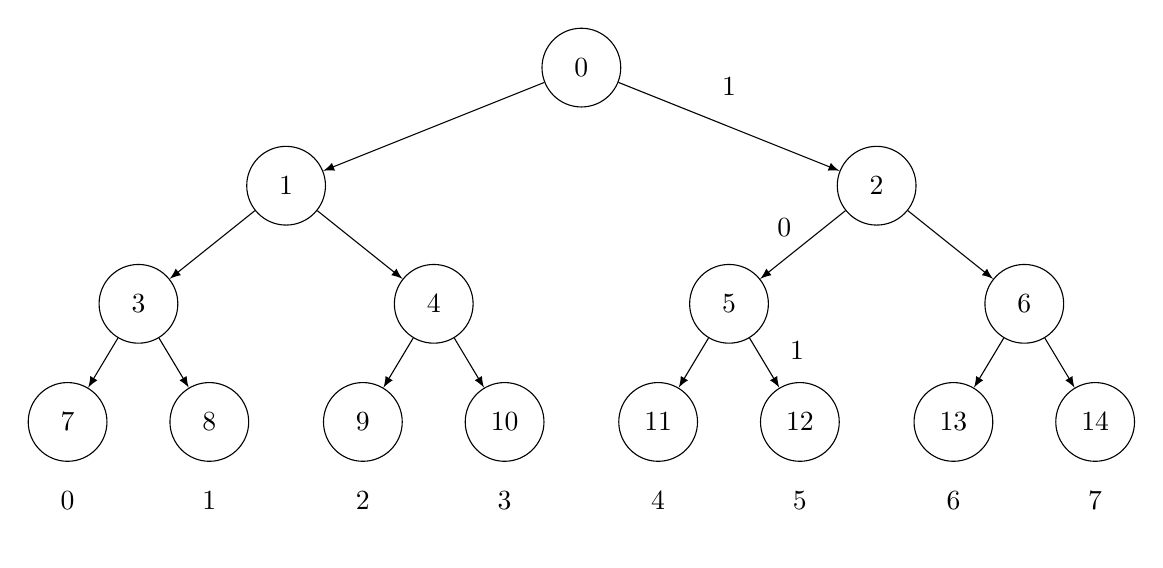
\begin{tikzpicture}[level/.style={sibling distance=75mm/#1},
        level 3/.style={sibling distance=18mm},
        every node/.style={minimum size=10mm,shape=circle},
        edge from parent/.style={draw,-latex}]
        \node[draw,grow=down] {0} 
        child {
          node[draw] {1}
          child { node[draw] {3}
            child {
              node[draw] (n7) {7}
            }
            child { node[draw] (n8) {8} }
          }
          child { node[draw] {4} 
            child { node[draw] (n9) {9} }
            child { node[draw] (n10) {10} }
          }
        }
        child {
          node[draw] {2}
          child { node[draw] {5}
            child { node[draw] (n11) {11} }
            child {
              node[draw] (n12) {12}
              edge from parent node[near start,right] {1}
            }
            edge from parent node[near start,left] {0}
          }
          child { node[draw] {6} 
            child { node[draw] (n13) {13} }
            child { node[draw] (n14) {14} }
          }
          edge from parent node[above] {1}
        };
        \node [below of=n7] {0};
        \node [below of=n8] {1};
        \node [below of=n9] {2};
        \node [below of=n10] {3};
        \node [below of=n11] {4};
        \node [below of=n12] {5};
        \node [below of=n13] {6};
        \node [below of=n14] {7};
  \end{tikzpicture}
  \caption{Visualisation of \cref{alg:bucketaddress}}
  \label{fig:bucketaddress}
\end{figure}

With this plumbing in place, we can input/output data from the outside and the underlying block device. Now we can implement \cref{alg:access}. Remapping the blocks requires a call to a pseudo-random function, reading in the path adds the contents of each bucket to the stash, and writing new data looks up a block in the stash and gives it a new data value. The final part is lines 11-16. This is where we decide which blocks should be put into the path.

The naive implementation of this, and that suggested by \cref{alg:access}, loops through the stash and finds blocks such that the bucket at level $l$ on the path to leaf $\mathsf{position[a']}$ is the same as the bucket at level $l$ on the path to leaf $x$. There are two small optimisations we can make here. The first is to perform the position lookup only once, attaching positions to the blocks in a temporary data structure, avoiding repeated work at each level. The second avoids calculating the bucket addresses entirely. We can do this by noting that in order for the paths to two leaves to intersect at level $l$, the leaves must have the same first $l$ bits. Thus, we can perform a right bit shift on both $x$ and $\mathsf{position[a']}$ of $\mathtt{height} - l$ bits, and check for equality.

We now have a functioning ORAM functor, that can be used to augment a block device in any Mirage program. In \cref{subsec:recursion,subsec:statelessness} we look at optimisations and extensions to this ORAM construction, before moving onto to the further aims of the project.

\subsection{Recursion}
\label{subsec:recursion}

The essence of recursive ORAM, is that the position map of one ORAM is another ORAM. Thus, we can extend our original ORAM functor, parameterising it in the implementation of the position map. To do this we use a single interface, that is satisfied by both the in memory position map and the ORAM module. We can apply this new ORAM functor with the in memory position map module to get our original construction. However, we can now take this further, applying the functor again with the result of the first application, and this can be done to an arbitrary depth. This is an exhibition of the power of OCaml's module system.

We can use the method above to build the recursive ORAM module by hand, applying the functor $n + 1$ times for $n$ levels of recursion. However, it is better to have a more automatic solution, where the recursive module is built automatically based on the size of the data ORAM, ORAM$_0$. Our addresses are 64-bit integers, so they take 8 bytes of storage each. If ORAM$_0$ has size $N$ in blocks, and the size of each block is $B$ bytes, then one block in ORAM$_1$ being used as the position map for ORAM$_0$ can store $\chi = B / 8$ addresses. The number of blocks required for ORAM$_1$ will therefore be $N / \chi$. After $\log N / \log \chi$ recursions, we will have a constant sized position map.

So, to create a recursive ORAM, we take in the size, $N$, and the block size, $B$, and automatically apply the ORAM functor recursively $\log N / \log \chi$ times. Calling the $\mathtt{create}$ function of the resulting module will create ORAM instances with the correct number of levels of recursion.

\subsection{Statelessness}
\label{subsec:statelessness}

In order to achieve statelessness for ORAM, we need to store type information, the stash, and the position map. We will first talk about how to layout all of this information on disk, before moving on to talk about how we actually get it there.

Once we have initialised ORAM and begun to use it, we do not want to move it around on disk, because we would have to copy the whole data structure. We do however need to store the information necessary to discover ORAMs existence in a well-known location, in order to allow us to reconnect to it. This leads us to storing a what is called a superblock in the first block of the underlying block device. This block will contain a pointer to the location of the rest of the state, along with its length. This way, we can store ORAM starting at the second location on disk, and then append all of the state at the end of the ORAM section, meaning we will never have to move ORAM once we have initialised it.

Now we actually need to store the state, which means we need some method of serialising it, ready to be written to disk. We could implement this manually, but for the majority of the information we can take advantage of an existing serialisation library, Jane Street's Bin\_prot. This is a binary protocol, that allows you to annotate a type with \texttt{[@@ deriving bin\_io]} and will then generate functions to read and write instances of the type into buffers. We are able to use this for all of the type information for ORAM, as well as for the stash. This leads us to splitting the ORAM type into a core, that can use Bin\_prot, and an extended type, that includes the position map and the underlying block device. This structure is shown in \cref{lst:orammaketype}.

The position map is more difficult to serialise, because under recursive ORAM, it might actually be another ORAM. We don't want to write the entire of the position map ORAM onto the disk a second time, so we need a custom serialisation function for the position map that will store only meta-data for ORAM position maps, and will store the entire position map in the base case. We want to store all state right at the end of the block device, after all recursive instances, so this function actually collects the data from all the levels of recursion together into one buffer.

Now that we can write all of the major parts into the buffer, we collect everything together and flush it to the end of the block device. After this is done, we are able to disconnect from ORAM safely. Reconnecting to ORAM is now a case of checking for the presence of the superblock, reading in the location and length of the state, reading the actual state, and then calling the connect function on the position map. The connect function allows each recursive ORAM instance to have its own reference to the underlying block device and returns once it reaches the in memory position map.

\section{File System}
\label{sec:fileSystem}

In order to search over documents, we first need some way of storing those documents. This section describes the design and implementation of a basic file system that satisfies the requirements of the project.

\subsection{General Design}

The most common way of building a file system on top of a block device is through the use of inodes. An inode contains meta-information about a file along with pointers to the actual data blocks. For the purposes of this project, an inode will simply be one sector of the block device, containing the length of the file, followed by the list of pointers. In a system with more complex needs the inode would contain more information, such as modification/access timestamps, file permissions, etc., but we simply want to be able to read and write documents.

We need to be able to access the inode for a particular file quickly, so we should store its location in an index. We could perform lookup based on the actual filename, but the names have variable lengths, therefore, because we want to store the index, it is better to lookup based on the hash of the filename. In a real system we would need to deal with collisions in the hash function, but for a small number of files we can neglect this possibility. \Cref{subsec:inodeindex} describes the implementation of the Inode Index.

We also need to allocate space on the block device for inode index blocks, for inode blocks and for data blocks, so we need a free map. This is a map that tells us which blocks on the device are free and allows us to update it as new blocks are needed. \Cref{subsec:freemap} describes the implementation of the free map.

We also want our file system to be stateless, and in order to do that, we need to store the data structures, along with enough information to find them on disk. We only need to store the root address of the Inode Index and the length of the Free Map to locate the data structures on disk when reconnecting to the block device. We store these two pieces of information at address 0 in another superblock.

\subsection{Inode Index}
\label{subsec:inodeindex}

We need a data structure that associates keys, in the form of file hashes, with values, in the form of pointers to inodes. We want to support operations of insertion, lookup and deletion efficiently, but we also want to store the data structure on disk. This leads us naturally to an implementation using B-Trees.\footnote{The algorithms for B-Tree operations were adapted from \citet{CLRS09}}

B-Trees are a generalisation of self-balancing binary search trees, where each node can have more than one child. If a node has $n$ children, then it stores $n-1$ keys. It is guaranteed that $$ \forall m \leq n, k \in child_m, j \in child_{m+1} . k < key_m < j, $$ that is, a key is greater than all the keys to its left and less than all the keys to its right.

B-Trees are an efficient on-disk data structure, because we can use the whole of a block for one node. This gives us an extremely high branching factor, reducing the depth of the tree and therefore the number of blocks that we need to access in any single operation. On creation of the file system, we calculate the branching factor of the tree in order to fill as much of each block as possible with useful information.

\subsection{Free Map}
\label{subsec:freemap}

In order to allocate space efficiently, we can simply use an array of bits the size of the block device. We again want to have an on-disk data structure, or at least one that can easily be flushed to disk regularly. It was therefore beneficial to write my own bit array based on \texttt{Cstruct}s, rather than using a library implementation. This gives us the ability to write the whole structure directly onto the disk using the block device methods, without any cumbersome translation.

The \texttt{Cstruct} library performs data access in bytes. This leads us to \cref{alg:bitgetset} for getting and setting individual bits. To get the $n^{th}$ bit, we must get the $\frac{n}{8}^{th}$ byte and extract it from there. To do this, we calculate the index of the bit in the byte, shift a 1 to that position, and perform an and, masking that bit. Setting is a similar operation, but seeks to preserve the surrounding bits. To set a 1, we calculate the index of the bit in the byte, shift a 1 to that position, and perform an or, preserving all other bits. Setting a 0 is slightly trickier. We want to perform an and with a bit string that is 0 at the desired position and 1 everywhere else, but shifting fills empty bits with 0s. We can however use De Morgan's Law $$ a~\&\&~b = \neg (\neg a~||~\neg b) $$ to convert this to an operation involving a bit string that has a 1 at the desired position and 0s everywhere else.

\begin{algorithm}[t]
\caption{Getting and setting individual bits in a byte array}
\label{alg:bitgetset}
\begin{algorithmic}
\vskip 10pt
\Function{GetBit}{$\mathsf{index}$}
  \State $byte \gets \mathsf{byteArray[index]}$
  \State $shift \gets 7 - \mathsf{index} \bmod 8$
  \State \Return $byte >> shift~\&\&~1$
\EndFunction
\vskip 10pt
\Function{SetBit}{$\mathsf{index,boolean}$}
  \State $byte \gets \mathsf{byteArray[index]}$
  \State $shift \gets 7 - \mathsf{index} \bmod 8$
  \If{$\mathsf{boolean}$}
    \State $byte \gets byte~||~1 << shift$
  \Else
    \State $byte \gets \neg (\neg byte~||~1 << shift)$
  \EndIf
  \State $\mathsf{byteArray[index]} \gets byte$
\EndFunction
\vskip 10pt
\end{algorithmic}
\end{algorithm}

\section{Search Module}
\label{sec:searchmodule}

So we have our documents and we can access them without revealing which ones we are accessing. Now the final piece of the puzzle is actually performing search. We discuss building an inverted index, the data structure that will allow us to search efficiently, in \cref{subsec:invertedindex}. We then discuss the front-end of the whole application, the search API, in \cref{subsec:searchapi}.

\subsection{Inverted Index}
\label{subsec:invertedindex}

The basics of inverted indexes are discussed in \cref{sec:invertedindexintro}. As stated there, the index consists of two main structures, the dictionary and the postings. For the dictionary, we will use the most common implementation, a hash table. This provides us with $O(1)$ lookup and insertion, which are the main operations we will be performing. The postings are more flexible. In our implementation we want to store the file names, because they are not actually stored in the file system itself. We also want to perform intersection of postings lists, allowing us to perform conjunctive queries. Thus, we will use a hash set, a data structure built on top of a hash table, that stores a set of keys, and has the added benefit of keeping them unique for us.

Having decided on our data structure, we need to actually index files. As usual in this project, the files will be \texttt{Cstruct}s. So we have a number of steps to perform in order to process a file. We first convert the file to a string and immediately strip it of characters we do not need, including all punctuation. At this point we have a sequence of alphanumeric character strings, separated by spaces and newlines, so we can perform a split on these characters to get a list of words.

We could perform indexing now, adding the name of the current file to the postings list of every word in our list, but there are a couple of things that we want to do first. We do not want to store separate words for `run', `ran', `runs', and so on, so we will perform some linguistic preprocessing. We will perform stemming, which uses a set of rules to prune suffixes, mapping words onto a stem. We will do this using Porter's stemming algorithm \cite{porter1980algorithm}. I used a small open-source library implementation of this algorithm, ocaml-stemmer. This technique not only reduces the size of the index, but also arguably improves search, because now queries for `run' can automatically returns documents containing morphological derivations. Finally, we remove duplicates from our list of words, reducing insertion overhead, and put the entries into the index.

For our purposes we will only implement simple conjunctive queries, meaning we look for documents containing all of the words in a space separated query string. Now to search we perform the same preprocessing on the query string, performing lookup on each of the queries in turn and taking the big intersection of the resulting list of hash sets. In order to make this intersection operation efficient, we sort the list by order of hash set size. Then we can filter the smaller hash set by checking for membership in the larger hash set. This means we perform one constant time lookup for each member of the small set, rather than the large, giving a large performance boost, as this smaller set is monotonically decreasing.

\subsection{Keyword Search API}
\label{subsec:searchapi}

The final step in an end-to-end system is the API. We need to wrap file system access, indexing and search all into one module that provides a single point of entry for an encrypted search system.

We have three main operations that are the most important to support. Writing files, reading files, and searching over files. We will not be concerned with deleting files in this project, because they are not important for the evaluation of ORAM. 

Writing files is the most important step, because this is where the search module does the indexing. On write, we first write through to the file system, then index the file and finally flush the index to disk to make sure it persists. Reading files is simply a pass through to the file system and search makes calls to inverted index.

\section{Summary}
\label{sec:implSummary}

In this chapter I have discussed the implementation of all of the components of my system, including the important design decisions and trade-offs that were made. We have seen how to implement recursive Path ORAM in a way that allows it to plug into existing MirageOS programs, and we have seen how to build a file system and search operations on top of it.

We now move on to the important task of evaluation, where we make sure that I have implemented ORAM in a way that ensures functionality, performance, and security, and have therefore achieved the aims of the project.

\chapter{Evaluation}

This chapter explains the methodology used to ensure the correctness of the ORAM implementation, as well as analysing its performance and security properties. \Cref{sec:unitTests} discusses functional testing through the use of unit testing and randomised testing. \Cref{sec:performanceTesting} then goes on to discuss performance, and then finally we analyse the security of ORAM in \cref{sec:statisticalAnalysis}.

Overall, ORAM performed as expected in terms of functionality, performance, and security. It operated correctly, writing files and reading the same data back out. It continued to do so with the additions of statelessness, recursion, and encryption, so all parts of the system were functional separately and as a whole. In terms of performance, my implementation agreed with the theoretical bounds given in \citet{stefanov2013path}, which state $O(\log N)$ time overhead. Finally, statistical analysis showed that ORAM did indeed have a statistically random access pattern, ensuring the security of the implementation.

If I had had more time, I would have performed more evaluation, examining different parameters of ORAM such as bucket size, extending experiments to larger ORAM sizes, and analysing different metrics such as bandwidth usage. Unfortunately experiments on ORAM take in the order of a few days to initialise and then a further day to run, so despite having a large amount of time to perform experiments, the nature of them restricted the amount that I could achieve.

\section{Unit Tests}
\label{sec:unitTests}

Unit testing was used throughout the development process, which allowed me to be sure that individual components were functioning correctly, before I combined them into larger more complicated systems. This section describes the most important test cases that were examined for each module and discusses the use of randomised testing to cover a larger range of input values. Code coverage testing was also used to make sure that the tests were visiting all parts of the system.

\subsection{Stash}

There are three main cases to test for the stash:

\begin{itemize}
  \item Values not expected to be in the stash are not found
  \item Values that have been added to the stash are found
  \item Adding dummy blocks to the stash has no effect
\end{itemize}

During the development process, I hand-coded a small number of example cases, but in order to test more extensively, I coded the above three cases as properties for randomised testing. This generates a number of test cases and verifies that the properties hold in every case and allows us to cover far more cases than hand-coded tests alone.

\subsection{Position Map}

We need to test the two main aspect of the position map. Firstly, the translation of 64 bit addresses into 3 regular integers, and then its actually operation as a data structure.

The code performing the translation is essentially a mathematical definition in itself, so any property definition that we might use for randomised testing would probably just be the original code. Thus, in this instance we simply check a few hand chosen random cases, along with the important edge cases. The edge cases we want to check are the maximum, and minimum values, along with values either side of a change in the higher indices, that is values with output $(x,y,max\_int)$ and $(x,y+1,0)$, and similarly for the higher index.

In terms of operation, we want to check that on adding a value to the position map, we read back the same value, and that trying to add a value at an address outside of the allowed range results in an error. Both of these cases can be coded up as properties for randomised testing.

\subsection{ORAM}

The ORAM implementation is particularly amenable to randomised testing, because we tend to define inverse functions for most of its functionality. This makes it very easy to write properties for randomised testing of the form $f(f^{-1}(x)) = x$. This allows us to check that each stage of ORAM is operating correctly, from writing individual blocks, through writing entire paths, to writing entire files.

For other functions that were not so easy to code properties for, regular unit testing was used. These include reconnecting to ORAM to test statelessness, and performing simple calculations, such as computing the height for ORAM.

\subsection{Free Map}

The Free Map allocates blocks in the block device to be used by different parts of the file system. We need to make sure that on creation, it allocates the correct number of initial blocks, and then subsequently always allocates the correct number of blocks, if they are available, and only ever allocates blocks that are actually free.

During development, I used only a handful of test cases, covering some of the most important edge cases. This included creating the map, and checking that nothing was allocated to begin with except the first $n$, where $n$ is passed into the creation function. Then, I checked that allocating and deallocating a few different sequences of blocks led to the expected results. Finally, I checked that if there were not enough free blocks, that an error was returned.

After main development had finished, I added some randomised testing to this module to cover a wider range of inputs.

\subsection{B-Trees}

It is not possible to test the B-Tree library directly, because it only gives us a functor to create a B-Tree. Thus the B-Tree was tested using the Inode Index, the canonical use case of the library in this system. In order to test the B-Tree properly, it was necessary to use randomised testing to create a reasonable access pattern that was guaranteed to cause splitting of the root node.

\subsection{Inodes}

The inodes needed to be tested to make sure they could add and delete pointers, while maintaining a correct count. This is again amenable to randomised testing, although unit tests were also used throughout the development to test specific cases that would be expected to cause exceptions.

\subsection{File System}

In order to test the file system I created a large number of random files and used randomised testing to ensure that under any access pattern the correct files were always read back out once they had been written in. This also included testing to ensure that reasonable exceptions were produced when the file system became full, or a file did not exist in the system.

\subsection{Search Module}

The search module was tested for correctness, i.e. if a file containing a word had been put into the system, then it would appear in the search results. This was difficult to randomise, so I manually constructed a number of test scenarios.

\section{Performance Testing}
\label{sec:performanceTesting}

\subsection{Parameter Optimisation}
\label{sub:parameterOptimisation}

Before performing the main experiments, I decided to optimise the parameters of ORAM, in order to allow the experiments to run faster. The main parameter in question is the block size, which has been shown in \citet{ousterhout1985trace} to dramatically affect the speed of IO operations. I discovered that this was indeed the case with ORAM, as can be seen in \cref{fig:blockSizeResults}. It appeared that increasing the block size has an unbounded increase on performance, but I settled with a block size of 1MB to trade-off between speed and the possibility to specify the size the block device.

It is important to note that using this in the cloud, we would see very different results. Increasing the block size will increase the size of the stash proportionally, because the maximum stash size is a constant number of blocks. Thus, a larger block size increases the amount of data that we must write to disk in order to achieve statelessness. We have shown that increasing block size increases speed when using a local disk, but network latency will dominate when running in the cloud, leading to a slow down. I would need to perform further experiments in the cloud to discover an optimal trade off point for this scenario.

\begin{figure}
    \centering
    %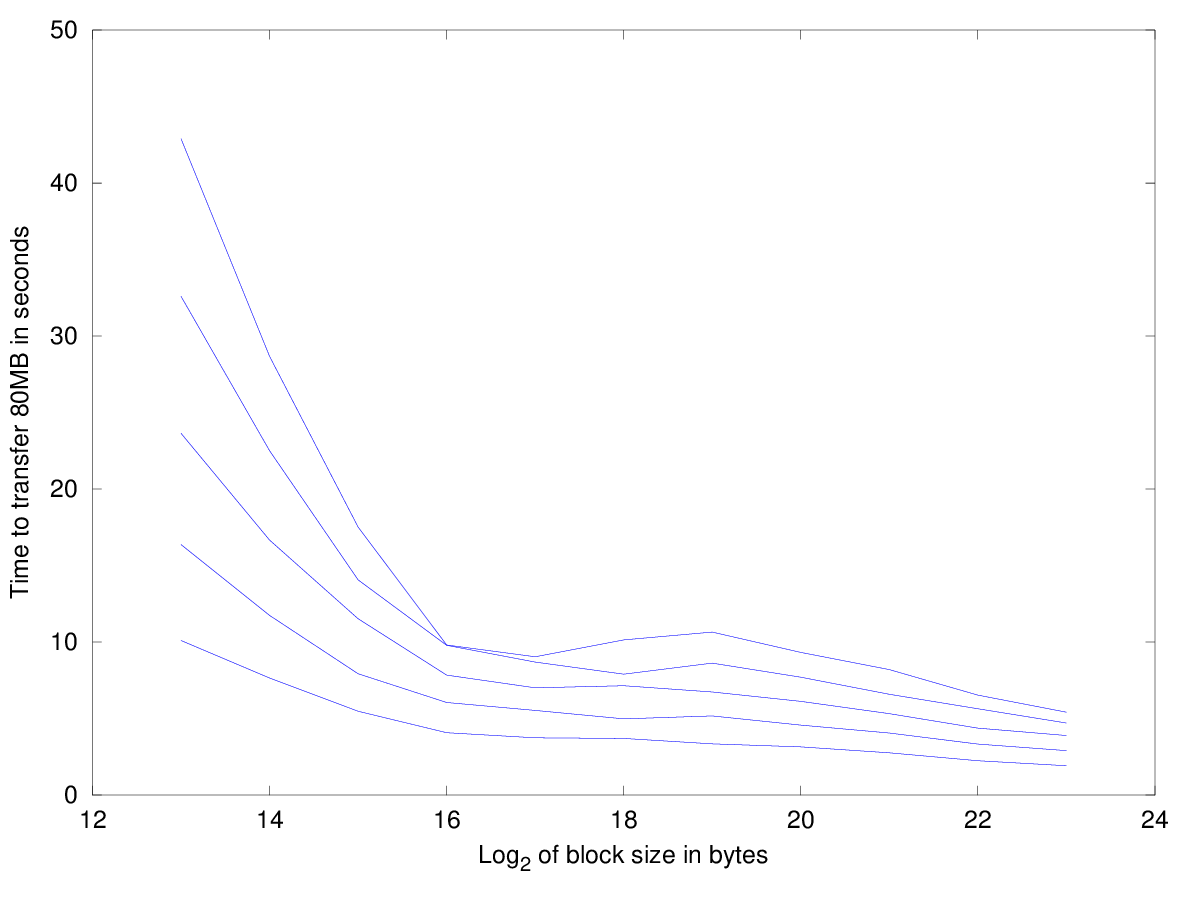
\includegraphics[width=.8\linewidth]{blockSizeResults}
    \input{blockSizeResults.tikz}
    \caption{Plot of the time taken to transfer 80MB of data at varying block sizes and sizes of ORAM. Each line represents one ORAM size, so we can see that as block size increases, the time decreases.}
    \label{fig:blockSizeResults}
\end{figure}

\subsection{Comparison with Literature}
\label{subsec:comparisonWithLiterature}

In order to effectively test the overhead due to ORAM, two things needed to be done very carefully. The first was isolating and removing major sources of uncertainty. When I first ran the experiments, I attempted to run them on my local machine. In this environment, other processes interfered with the ORAM process, making the results unreliable. I secured a remote testing machine in order to run the experiments in complete isolation. Here, at first, they were running on an NFS mounted drive, meaning that network latency and protocol overheads were affecting the results. After moving the experiments to local disk, it was clear that ORAM overheads were finally dominating the results. Now, secondly, I needed to initialise the ORAMs properly. Using a fresh ORAM, the stash is empty and most of the blocks are dummy blocks that get disregarded. It is necessary to run an initialisation sequence in order to remove the effects of these on the results. We use the worst case sequence, writing each block in turn, then reading each block in turn, to ensure that all blocks get used multiple times, leaving the ORAM in a state that it would likely be in after extended use. Only once this steady state has been reached can we reliably test the performance.

For the actual experiment, rather than using the worst case sequence, we use a random sequence of block accesses. We perform 10 runs of 1000 iterations each, oscillating between reads and writes in order to balance the different overheads. We are trying to see how the performance changes as the block size increases, so we use ORAMs of a range of sizes, from 12 blocks (a tree of depth 1) to 4092 blocks (a tree of depth 9). The log of the time taken for each ORAM to perform 1000 iterations is plotted against the logarithm of the size of the ORAM in \cref{fig:timeResults}. We expect this to be a straight line, because we expect logarithmic overheads from ORAM, and we increase the block sizes roughly in powers of two. We can see that ORAM does indeed show a logarithm overhead compared to the control experiment that performed the same sequence of accesses to a block device without ORAM. I performed the same experiment adding encryption to ORAM and we can see that the overhead was still logarithmic, but with a larger constant.

\begin{figure}
    \centering
    %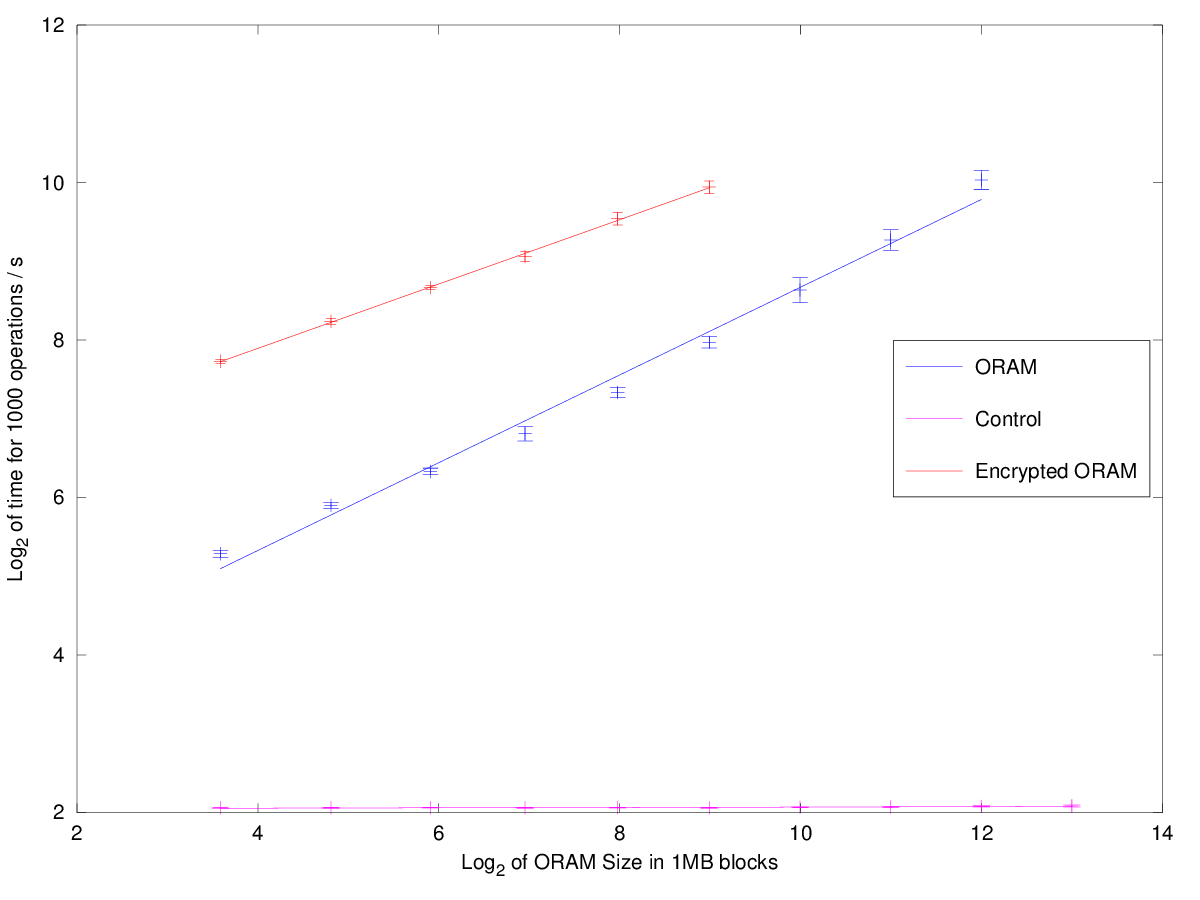
\includegraphics[width=.8\linewidth]{timeResults}
    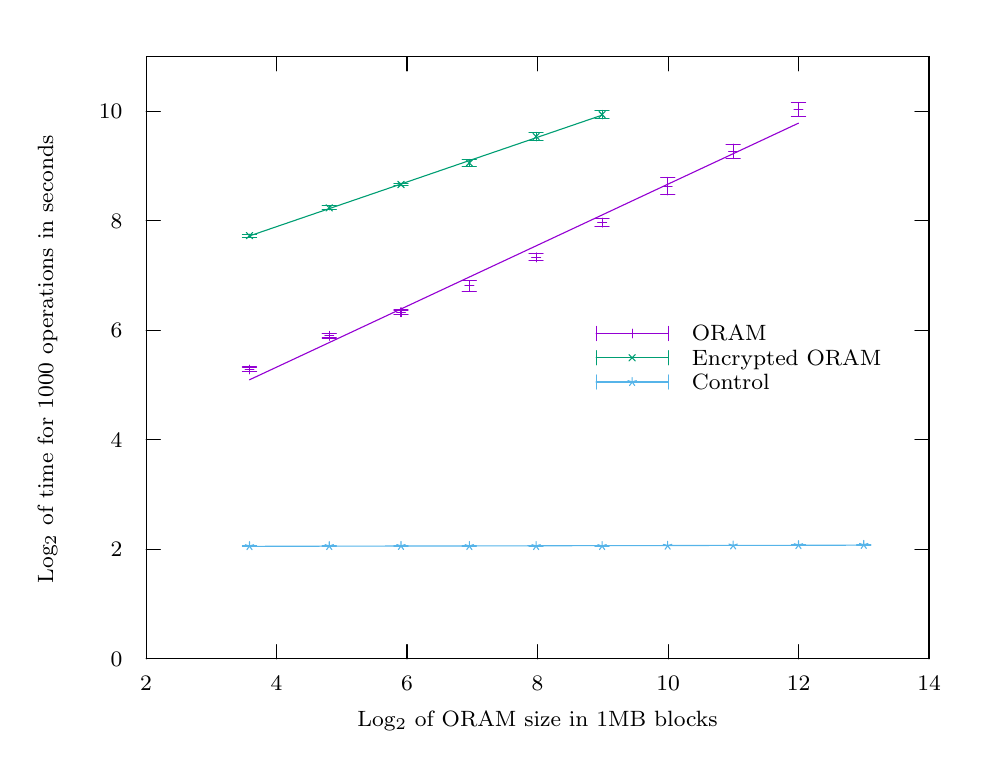
\begin{tikzpicture}[gnuplot]
%% generated with GNUPLOT 5.0p3 (Lua 5.3; terminal rev. 99, script rev. 100)
%% Mon 02 May 2016 10:36:46 BST
\path (0.000,0.000) rectangle (12.000,9.000);
\gpcolor{color=gp lt color border}
\gpsetlinetype{gp lt border}
\gpsetdashtype{gp dt solid}
\gpsetlinewidth{1.00}
\draw[gp path] (1.504,0.985)--(1.684,0.985);
\draw[gp path] (11.447,0.985)--(11.267,0.985);
\node[gp node right] at (1.320,0.985) {\footnotesize 0};
\draw[gp path] (1.504,2.375)--(1.684,2.375);
\draw[gp path] (11.447,2.375)--(11.267,2.375);
\node[gp node right] at (1.320,2.375) {\footnotesize 2};
\draw[gp path] (1.504,3.765)--(1.684,3.765);
\draw[gp path] (11.447,3.765)--(11.267,3.765);
\node[gp node right] at (1.320,3.765) {\footnotesize 4};
\draw[gp path] (1.504,5.156)--(1.684,5.156);
\draw[gp path] (11.447,5.156)--(11.267,5.156);
\node[gp node right] at (1.320,5.156) {\footnotesize 6};
\draw[gp path] (1.504,6.546)--(1.684,6.546);
\draw[gp path] (11.447,6.546)--(11.267,6.546);
\node[gp node right] at (1.320,6.546) {\footnotesize 8};
\draw[gp path] (1.504,7.936)--(1.684,7.936);
\draw[gp path] (11.447,7.936)--(11.267,7.936);
\node[gp node right] at (1.320,7.936) {\footnotesize 10};
\draw[gp path] (1.504,0.985)--(1.504,1.165);
\draw[gp path] (1.504,8.631)--(1.504,8.451);
\node[gp node center] at (1.504,0.677) {\footnotesize 2};
\draw[gp path] (3.161,0.985)--(3.161,1.165);
\draw[gp path] (3.161,8.631)--(3.161,8.451);
\node[gp node center] at (3.161,0.677) {\footnotesize 4};
\draw[gp path] (4.818,0.985)--(4.818,1.165);
\draw[gp path] (4.818,8.631)--(4.818,8.451);
\node[gp node center] at (4.818,0.677) {\footnotesize 6};
\draw[gp path] (6.476,0.985)--(6.476,1.165);
\draw[gp path] (6.476,8.631)--(6.476,8.451);
\node[gp node center] at (6.476,0.677) {\footnotesize 8};
\draw[gp path] (8.133,0.985)--(8.133,1.165);
\draw[gp path] (8.133,8.631)--(8.133,8.451);
\node[gp node center] at (8.133,0.677) {\footnotesize 10};
\draw[gp path] (9.790,0.985)--(9.790,1.165);
\draw[gp path] (9.790,8.631)--(9.790,8.451);
\node[gp node center] at (9.790,0.677) {\footnotesize 12};
\draw[gp path] (11.447,0.985)--(11.447,1.165);
\draw[gp path] (11.447,8.631)--(11.447,8.451);
\node[gp node center] at (11.447,0.677) {\footnotesize 14};
\draw[gp path] (1.504,8.631)--(1.504,0.985)--(11.447,0.985)--(11.447,8.631)--cycle;
\node[gp node center,rotate=-270] at (0.246,4.808) {\footnotesize Log$_2$ of time for 1000 operations in seconds};
\node[gp node center] at (6.475,0.215) {\footnotesize Log$_2$ of ORAM size in 1MB blocks};
\node[gp node left] at (8.319,5.116) {\footnotesize ORAM};
\gpcolor{rgb color={0.580,0.000,0.827}}
\draw[gp path] (7.219,5.116)--(8.135,5.116);
\draw[gp path] (7.219,5.206)--(7.219,5.026);
\draw[gp path] (8.135,5.206)--(8.135,5.026);
\draw[gp path] (2.817,4.629)--(2.817,4.690);
\draw[gp path] (2.727,4.629)--(2.907,4.629);
\draw[gp path] (2.727,4.690)--(2.907,4.690);
\draw[gp path] (3.830,5.059)--(3.830,5.113);
\draw[gp path] (3.740,5.059)--(3.920,5.059);
\draw[gp path] (3.740,5.113)--(3.920,5.113);
\draw[gp path] (4.741,5.356)--(4.741,5.415);
\draw[gp path] (4.651,5.356)--(4.831,5.356);
\draw[gp path] (4.651,5.415)--(4.831,5.415);
\draw[gp path] (5.609,5.655)--(5.609,5.785);
\draw[gp path] (5.519,5.655)--(5.699,5.655);
\draw[gp path] (5.519,5.785)--(5.699,5.785);
\draw[gp path] (6.457,6.039)--(6.457,6.127);
\draw[gp path] (6.367,6.039)--(6.547,6.039);
\draw[gp path] (6.367,6.127)--(6.547,6.127);
\draw[gp path] (7.295,6.476)--(7.295,6.575);
\draw[gp path] (7.205,6.476)--(7.385,6.476);
\draw[gp path] (7.205,6.575)--(7.385,6.575);
\draw[gp path] (8.128,6.876)--(8.128,7.099);
\draw[gp path] (8.038,6.876)--(8.218,6.876);
\draw[gp path] (8.038,7.099)--(8.218,7.099);
\draw[gp path] (8.959,7.338)--(8.959,7.520);
\draw[gp path] (8.869,7.338)--(9.049,7.338);
\draw[gp path] (8.869,7.520)--(9.049,7.520);
\draw[gp path] (9.789,7.876)--(9.789,8.044);
\draw[gp path] (9.699,7.876)--(9.879,7.876);
\draw[gp path] (9.699,8.044)--(9.879,8.044);
\gpsetpointsize{4.00}
\gppoint{gp mark 1}{(2.817,4.659)}
\gppoint{gp mark 1}{(3.830,5.086)}
\gppoint{gp mark 1}{(4.741,5.386)}
\gppoint{gp mark 1}{(5.609,5.720)}
\gppoint{gp mark 1}{(6.457,6.083)}
\gppoint{gp mark 1}{(7.295,6.525)}
\gppoint{gp mark 1}{(8.128,6.987)}
\gppoint{gp mark 1}{(8.959,7.429)}
\gppoint{gp mark 1}{(9.789,7.960)}
\gppoint{gp mark 1}{(7.677,5.116)}
\draw[gp path] (2.817,4.528)--(3.830,5.001)--(4.741,5.427)--(5.609,5.833)--(6.457,6.229)%
  --(7.295,6.621)--(8.128,7.011)--(8.959,7.399)--(9.789,7.787);
\gpcolor{color=gp lt color border}
\node[gp node left] at (8.319,4.808) {\footnotesize Encrypted ORAM};
\gpcolor{rgb color={0.000,0.620,0.451}}
\draw[gp path] (7.219,4.808)--(8.135,4.808);
\draw[gp path] (7.219,4.898)--(7.219,4.718);
\draw[gp path] (8.135,4.898)--(8.135,4.718);
\draw[gp path] (2.817,6.340)--(2.817,6.377);
\draw[gp path] (2.727,6.340)--(2.907,6.340);
\draw[gp path] (2.727,6.377)--(2.907,6.377);
\draw[gp path] (3.830,6.686)--(3.830,6.738);
\draw[gp path] (3.740,6.686)--(3.920,6.686);
\draw[gp path] (3.740,6.738)--(3.920,6.738);
\draw[gp path] (4.741,6.993)--(4.741,7.024);
\draw[gp path] (4.651,6.993)--(4.831,6.993);
\draw[gp path] (4.651,7.024)--(4.831,7.024);
\draw[gp path] (5.609,7.238)--(5.609,7.326);
\draw[gp path] (5.519,7.238)--(5.699,7.238);
\draw[gp path] (5.519,7.326)--(5.699,7.326);
\draw[gp path] (6.457,7.563)--(6.457,7.671);
\draw[gp path] (6.367,7.563)--(6.547,7.563);
\draw[gp path] (6.367,7.671)--(6.547,7.671);
\draw[gp path] (7.295,7.842)--(7.295,7.950);
\draw[gp path] (7.205,7.842)--(7.385,7.842);
\draw[gp path] (7.205,7.950)--(7.385,7.950);
\gppoint{gp mark 2}{(2.817,6.358)}
\gppoint{gp mark 2}{(3.830,6.712)}
\gppoint{gp mark 2}{(4.741,7.008)}
\gppoint{gp mark 2}{(5.609,7.282)}
\gppoint{gp mark 2}{(6.457,7.617)}
\gppoint{gp mark 2}{(7.295,7.896)}
\gppoint{gp mark 2}{(7.677,4.808)}
\draw[gp path] (2.817,6.355)--(3.830,6.702)--(4.741,7.014)--(5.609,7.312)--(6.457,7.602)%
  --(7.295,7.889);
\gpcolor{color=gp lt color border}
\node[gp node left] at (8.319,4.500) {\footnotesize Control};
\gpcolor{rgb color={0.337,0.706,0.914}}
\draw[gp path] (7.219,4.500)--(8.135,4.500);
\draw[gp path] (7.219,4.590)--(7.219,4.410);
\draw[gp path] (8.135,4.590)--(8.135,4.410);
\draw[gp path] (2.817,2.413)--(2.817,2.419);
\draw[gp path] (2.727,2.413)--(2.907,2.413);
\draw[gp path] (2.727,2.419)--(2.907,2.419);
\draw[gp path] (3.830,2.414)--(3.830,2.419);
\draw[gp path] (3.740,2.414)--(3.920,2.414);
\draw[gp path] (3.740,2.419)--(3.920,2.419);
\draw[gp path] (4.741,2.415)--(4.741,2.420);
\draw[gp path] (4.651,2.415)--(4.831,2.415);
\draw[gp path] (4.651,2.420)--(4.831,2.420);
\draw[gp path] (5.609,2.414)--(5.609,2.420);
\draw[gp path] (5.519,2.414)--(5.699,2.414);
\draw[gp path] (5.519,2.420)--(5.699,2.420);
\draw[gp path] (6.457,2.416)--(6.457,2.419);
\draw[gp path] (6.367,2.416)--(6.547,2.416);
\draw[gp path] (6.367,2.419)--(6.547,2.419);
\draw[gp path] (7.295,2.413)--(7.295,2.420);
\draw[gp path] (7.205,2.413)--(7.385,2.413);
\draw[gp path] (7.205,2.420)--(7.385,2.420);
\draw[gp path] (8.128,2.418)--(8.128,2.424);
\draw[gp path] (8.038,2.418)--(8.218,2.418);
\draw[gp path] (8.038,2.424)--(8.218,2.424);
\draw[gp path] (8.959,2.419)--(8.959,2.428);
\draw[gp path] (8.869,2.419)--(9.049,2.419);
\draw[gp path] (8.869,2.428)--(9.049,2.428);
\draw[gp path] (9.789,2.425)--(9.789,2.434);
\draw[gp path] (9.699,2.425)--(9.879,2.425);
\draw[gp path] (9.699,2.434)--(9.879,2.434);
\draw[gp path] (10.618,2.423)--(10.618,2.440);
\draw[gp path] (10.528,2.423)--(10.708,2.423);
\draw[gp path] (10.528,2.440)--(10.708,2.440);
\gppoint{gp mark 3}{(2.817,2.416)}
\gppoint{gp mark 3}{(3.830,2.417)}
\gppoint{gp mark 3}{(4.741,2.418)}
\gppoint{gp mark 3}{(5.609,2.417)}
\gppoint{gp mark 3}{(6.457,2.417)}
\gppoint{gp mark 3}{(7.295,2.417)}
\gppoint{gp mark 3}{(8.128,2.421)}
\gppoint{gp mark 3}{(8.959,2.424)}
\gppoint{gp mark 3}{(9.789,2.429)}
\gppoint{gp mark 3}{(10.618,2.432)}
\gppoint{gp mark 3}{(7.677,4.500)}
\draw[gp path] (2.817,2.413)--(3.830,2.415)--(4.741,2.417)--(5.609,2.418)--(6.457,2.420)%
  --(7.295,2.422)--(8.128,2.423)--(8.959,2.425)--(9.789,2.426)--(10.618,2.428);
\gpcolor{color=gp lt color border}
\draw[gp path] (1.504,8.631)--(1.504,0.985)--(11.447,0.985)--(11.447,8.631)--cycle;
%% coordinates of the plot area
\gpdefrectangularnode{gp plot 1}{\pgfpoint{1.504cm}{0.985cm}}{\pgfpoint{11.447cm}{8.631cm}}
\end{tikzpicture}

    \caption{The relationship between size of an ORAM in blocks and the time taken for 1000 operations, plotted for ORAM, encrypted ORAM, and a control block device with no ORAM. We take logs of both axes, because block size was increased in powers of two and we expect a log relationship.}
    \label{fig:timeResults}
\end{figure}

%The initialisation phase allowed the stash size to reach a steady state, which resulted in a constant overhead of $x$ blocks, compared with $y$ predicted in \citet{stefanov2013path} for a security parameter, $\lambda = z$. This shows something...

%In these first experiments, we used stateless, non-recursive ORAM, which means that the entire of the position map was being flushed to disk on every access. We now compare the time taken for stateless, recursive ORAM, to see what effect the additional recursive calls have compared to the reduction in the size of the client side state. We can see from \cref{fig:recursiveTimePlot} that overall this was good/bad to some degree.

Although it has not been discussed here, bandwidth is another important measure when examining the performance of ORAM, especially when it is being used in the cloud. With more time, a detailed study of the bandwidth used with and without recursion would have been carried out, which would have given further insight into the trade-off that recursion presents us with.

\section{Statistical Analysis}
\label{sec:statisticalAnalysis}

In order to test the effectiveness of ORAM, we need to show that the access pattern observed by the block device is actually statistically random. Of course there is structure to this randomness, because on each access a whole path is read and written, but the actual path that gets written should be random. Thus, we should perform a test for randomness on a sequence of path indices.

In order to do this we will use two common techniques: autocorrelation plotting and runs testing.

Autocorrelation plotting plots the correlation of a sequence with itself at various time lags \cite{nistautocorr}. For a random sequence the noise cancels itself out, so we want to see a plot of values very close to zero, apart from at lag 0, where the correlation will be exactly the power of the signal. I plotted this for two access patterns, one of length 200 so that the results would be easily visible, and one of length 5,000 to show longer term effects. For both of these patterns, the underlying access pattern, the one that would be seen without ORAM, was simply a succession of reads and writes to the same location. These plots are shown in \cref{fig:shortAutocorr} and \cref{fig:longAutocorr} respectively.

\begin{figure}
    \centering
    \begin{subfigure}{.45\textwidth}
        \centering
        %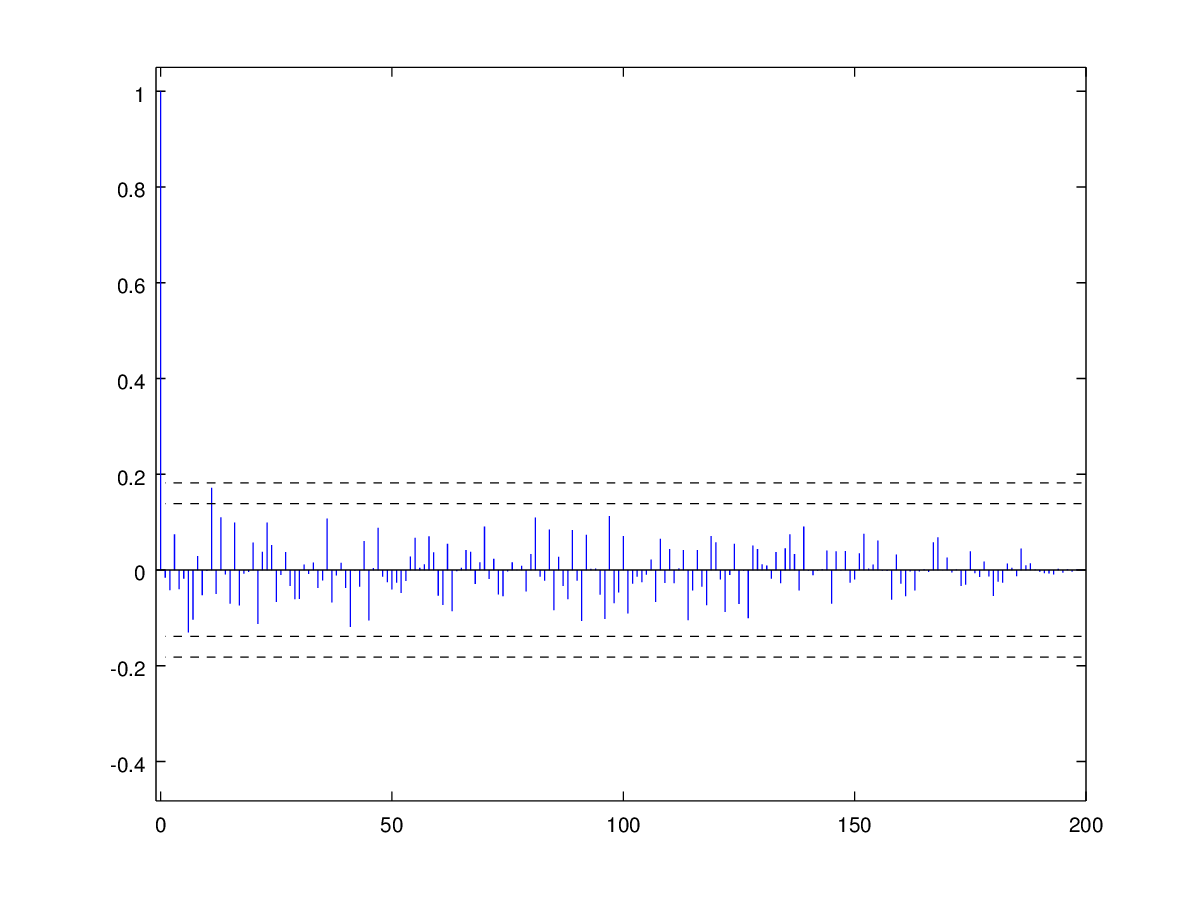
\includegraphics[width=\linewidth]{shortAutocorr}
        \scalebox{0.9}{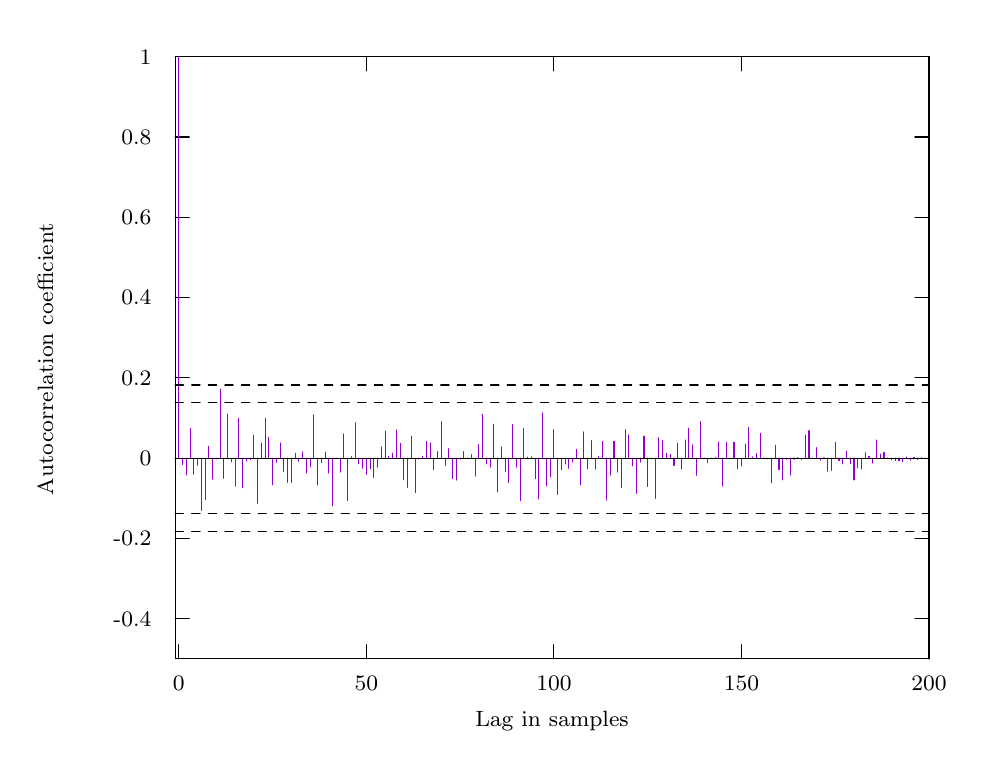
\begin{tikzpicture}[gnuplot]
%% generated with GNUPLOT 5.0p3 (Lua 5.3; terminal rev. 99, script rev. 100)
%% Mon 02 May 2016 08:41:38 BST
\path (0.000,0.000) rectangle (12.000,9.000);
\gpcolor{color=gp lt color border}
\gpsetlinetype{gp lt border}
\gpsetdashtype{gp dt solid}
\gpsetlinewidth{1.00}
\draw[gp path] (1.872,1.495)--(2.052,1.495);
\draw[gp path] (11.447,1.495)--(11.267,1.495);
\node[gp node right] at (1.688,1.495) {\footnotesize -0.4};
\draw[gp path] (1.872,2.514)--(2.052,2.514);
\draw[gp path] (11.447,2.514)--(11.267,2.514);
\node[gp node right] at (1.688,2.514) {\footnotesize -0.2};
\draw[gp path] (1.872,3.534)--(2.052,3.534);
\draw[gp path] (11.447,3.534)--(11.267,3.534);
\node[gp node right] at (1.688,3.534) {\footnotesize 0};
\draw[gp path] (1.872,4.553)--(2.052,4.553);
\draw[gp path] (11.447,4.553)--(11.267,4.553);
\node[gp node right] at (1.688,4.553) {\footnotesize 0.2};
\draw[gp path] (1.872,5.573)--(2.052,5.573);
\draw[gp path] (11.447,5.573)--(11.267,5.573);
\node[gp node right] at (1.688,5.573) {\footnotesize 0.4};
\draw[gp path] (1.872,6.592)--(2.052,6.592);
\draw[gp path] (11.447,6.592)--(11.267,6.592);
\node[gp node right] at (1.688,6.592) {\footnotesize 0.6};
\draw[gp path] (1.872,7.612)--(2.052,7.612);
\draw[gp path] (11.447,7.612)--(11.267,7.612);
\node[gp node right] at (1.688,7.612) {\footnotesize 0.8};
\draw[gp path] (1.872,8.631)--(2.052,8.631);
\draw[gp path] (11.447,8.631)--(11.267,8.631);
\node[gp node right] at (1.688,8.631) {\footnotesize 1};
\draw[gp path] (1.920,0.985)--(1.920,1.165);
\draw[gp path] (1.920,8.631)--(1.920,8.451);
\node[gp node center] at (1.920,0.677) {\footnotesize 0};
\draw[gp path] (4.301,0.985)--(4.301,1.165);
\draw[gp path] (4.301,8.631)--(4.301,8.451);
\node[gp node center] at (4.301,0.677) {\footnotesize 50};
\draw[gp path] (6.683,0.985)--(6.683,1.165);
\draw[gp path] (6.683,8.631)--(6.683,8.451);
\node[gp node center] at (6.683,0.677) {\footnotesize 100};
\draw[gp path] (9.065,0.985)--(9.065,1.165);
\draw[gp path] (9.065,8.631)--(9.065,8.451);
\node[gp node center] at (9.065,0.677) {\footnotesize 150};
\draw[gp path] (11.447,0.985)--(11.447,1.165);
\draw[gp path] (11.447,8.631)--(11.447,8.451);
\node[gp node center] at (11.447,0.677) {\footnotesize 200};
\draw[gp path] (1.872,8.631)--(1.872,0.985)--(11.447,0.985)--(11.447,8.631)--cycle;
\node[gp node center,rotate=-270] at (0.246,4.808) {\footnotesize Autocorrelation coefficient};
\node[gp node center] at (6.659,0.215) {\footnotesize Lag in samples};
\gpcolor{rgb color={0.580,0.000,0.827}}
\draw[gp path] (1.920,3.534)--(1.920,8.631);
\draw[gp path] (1.967,3.534)--(1.967,3.452);
\draw[gp path] (2.015,3.534)--(2.015,3.320);
\draw[gp path] (2.063,3.534)--(2.063,3.912);
\draw[gp path] (2.110,3.534)--(2.110,3.330);
\draw[gp path] (2.158,3.534)--(2.158,3.443);
\draw[gp path] (2.205,3.534)--(2.205,2.870);
\draw[gp path] (2.253,3.534)--(2.253,3.007);
\draw[gp path] (2.301,3.534)--(2.301,3.682);
\draw[gp path] (2.348,3.534)--(2.348,3.267);
\draw[gp path] (2.396,3.534)--(2.396,3.524);
\draw[gp path] (2.444,3.534)--(2.444,4.408);
\draw[gp path] (2.491,3.534)--(2.491,3.278);
\draw[gp path] (2.539,3.534)--(2.539,4.093);
\draw[gp path] (2.587,3.534)--(2.587,3.487);
\draw[gp path] (2.634,3.534)--(2.634,3.177);
\draw[gp path] (2.682,3.534)--(2.682,4.037);
\draw[gp path] (2.729,3.534)--(2.729,3.158);
\draw[gp path] (2.777,3.534)--(2.777,3.495);
\draw[gp path] (2.825,3.534)--(2.825,3.514);
\draw[gp path] (2.872,3.534)--(2.872,3.825);
\draw[gp path] (2.920,3.534)--(2.920,2.960);
\draw[gp path] (2.968,3.534)--(2.968,3.727);
\draw[gp path] (3.015,3.534)--(3.015,4.039);
\draw[gp path] (3.063,3.534)--(3.063,3.799);
\draw[gp path] (3.111,3.534)--(3.111,3.195);
\draw[gp path] (3.158,3.534)--(3.158,3.483);
\draw[gp path] (3.206,3.534)--(3.206,3.725);
\draw[gp path] (3.253,3.534)--(3.253,3.365);
\draw[gp path] (3.301,3.534)--(3.301,3.225);
\draw[gp path] (3.349,3.534)--(3.349,3.227);
\draw[gp path] (3.396,3.534)--(3.396,3.592);
\draw[gp path] (3.444,3.534)--(3.444,3.494);
\draw[gp path] (3.492,3.534)--(3.492,3.613);
\draw[gp path] (3.539,3.534)--(3.539,3.345);
\draw[gp path] (3.587,3.534)--(3.587,3.423);
\draw[gp path] (3.635,3.534)--(3.635,4.081);
\draw[gp path] (3.682,3.534)--(3.682,3.190);
\draw[gp path] (3.730,3.534)--(3.730,3.477);
\draw[gp path] (3.777,3.534)--(3.777,3.609);
\draw[gp path] (3.825,3.534)--(3.825,3.344);
\draw[gp path] (3.873,3.534)--(3.873,2.928);
\draw[gp path] (3.920,3.534)--(3.920,3.526);
\draw[gp path] (3.968,3.534)--(3.968,3.357);
\draw[gp path] (4.016,3.534)--(4.016,3.841);
\draw[gp path] (4.063,3.534)--(4.063,2.997);
\draw[gp path] (4.111,3.534)--(4.111,3.553);
\draw[gp path] (4.159,3.534)--(4.159,3.982);
\draw[gp path] (4.206,3.534)--(4.206,3.465);
\draw[gp path] (4.254,3.534)--(4.254,3.405);
\draw[gp path] (4.301,3.534)--(4.301,3.327);
\draw[gp path] (4.349,3.534)--(4.349,3.400);
\draw[gp path] (4.397,3.534)--(4.397,3.290);
\draw[gp path] (4.444,3.534)--(4.444,3.418);
\draw[gp path] (4.492,3.534)--(4.492,3.676);
\draw[gp path] (4.540,3.534)--(4.540,3.875);
\draw[gp path] (4.587,3.534)--(4.587,3.556);
\draw[gp path] (4.635,3.534)--(4.635,3.592);
\draw[gp path] (4.683,3.534)--(4.683,3.891);
\draw[gp path] (4.730,3.534)--(4.730,3.721);
\draw[gp path] (4.778,3.534)--(4.778,3.262);
\draw[gp path] (4.825,3.534)--(4.825,3.162);
\draw[gp path] (4.873,3.534)--(4.873,3.812);
\draw[gp path] (4.921,3.534)--(4.921,3.096);
\draw[gp path] (4.968,3.534)--(4.968,3.521);
\draw[gp path] (5.016,3.534)--(5.016,3.556);
\draw[gp path] (5.064,3.534)--(5.064,3.746);
\draw[gp path] (5.111,3.534)--(5.111,3.727);
\draw[gp path] (5.159,3.534)--(5.159,3.387);
\draw[gp path] (5.207,3.534)--(5.207,3.616);
\draw[gp path] (5.254,3.534)--(5.254,3.995);
\draw[gp path] (5.302,3.534)--(5.302,3.438);
\draw[gp path] (5.349,3.534)--(5.349,3.652);
\draw[gp path] (5.397,3.534)--(5.397,3.274);
\draw[gp path] (5.445,3.534)--(5.445,3.255);
\draw[gp path] (5.492,3.534)--(5.492,3.520);
\draw[gp path] (5.540,3.534)--(5.540,3.616);
\draw[gp path] (5.588,3.534)--(5.588,3.536);
\draw[gp path] (5.635,3.534)--(5.635,3.577);
\draw[gp path] (5.683,3.534)--(5.683,3.305);
\draw[gp path] (5.731,3.534)--(5.731,3.703);
\draw[gp path] (5.778,3.534)--(5.778,4.092);
\draw[gp path] (5.826,3.534)--(5.826,3.462);
\draw[gp path] (5.873,3.534)--(5.873,3.420);
\draw[gp path] (5.921,3.534)--(5.921,3.963);
\draw[gp path] (5.969,3.534)--(5.969,3.105);
\draw[gp path] (6.016,3.534)--(6.016,3.674);
\draw[gp path] (6.064,3.534)--(6.064,3.364);
\draw[gp path] (6.112,3.534)--(6.112,3.224);
\draw[gp path] (6.159,3.534)--(6.159,3.957);
\draw[gp path] (6.207,3.534)--(6.207,3.420);
\draw[gp path] (6.255,3.534)--(6.255,2.993);
\draw[gp path] (6.302,3.534)--(6.302,3.908);
\draw[gp path] (6.350,3.534)--(6.350,3.545);
\draw[gp path] (6.397,3.534)--(6.397,3.549);
\draw[gp path] (6.445,3.534)--(6.445,3.272);
\draw[gp path] (6.493,3.534)--(6.493,3.015);
\draw[gp path] (6.540,3.534)--(6.540,4.108);
\draw[gp path] (6.588,3.534)--(6.588,3.182);
\draw[gp path] (6.636,3.534)--(6.636,3.295);
\draw[gp path] (6.683,3.534)--(6.683,3.895);
\draw[gp path] (6.731,3.534)--(6.731,3.072);
\draw[gp path] (6.779,3.534)--(6.779,3.388);
\draw[gp path] (6.826,3.534)--(6.826,3.462);
\draw[gp path] (6.874,3.534)--(6.874,3.405);
\draw[gp path] (6.922,3.534)--(6.922,3.485);
\draw[gp path] (6.969,3.534)--(6.969,3.644);
\draw[gp path] (7.017,3.534)--(7.017,3.195);
\draw[gp path] (7.064,3.534)--(7.064,3.866);
\draw[gp path] (7.112,3.534)--(7.112,3.397);
\draw[gp path] (7.160,3.534)--(7.160,3.756);
\draw[gp path] (7.207,3.534)--(7.207,3.394);
\draw[gp path] (7.255,3.534)--(7.255,3.551);
\draw[gp path] (7.303,3.534)--(7.303,3.745);
\draw[gp path] (7.350,3.534)--(7.350,3.001);
\draw[gp path] (7.398,3.534)--(7.398,3.317);
\draw[gp path] (7.446,3.534)--(7.446,3.746);
\draw[gp path] (7.493,3.534)--(7.493,3.357);
\draw[gp path] (7.541,3.534)--(7.541,3.160);
\draw[gp path] (7.588,3.534)--(7.588,3.895);
\draw[gp path] (7.636,3.534)--(7.636,3.828);
\draw[gp path] (7.684,3.534)--(7.684,3.435);
\draw[gp path] (7.731,3.534)--(7.731,3.087);
\draw[gp path] (7.779,3.534)--(7.779,3.483);
\draw[gp path] (7.827,3.534)--(7.827,3.812);
\draw[gp path] (7.874,3.534)--(7.874,3.174);
\draw[gp path] (7.922,3.534)--(7.922,3.527);
\draw[gp path] (7.970,3.534)--(7.970,3.021);
\draw[gp path] (8.017,3.534)--(8.017,3.794);
\draw[gp path] (8.065,3.534)--(8.065,3.756);
\draw[gp path] (8.112,3.534)--(8.112,3.594);
\draw[gp path] (8.160,3.534)--(8.160,3.581);
\draw[gp path] (8.208,3.534)--(8.208,3.441);
\draw[gp path] (8.255,3.534)--(8.255,3.723);
\draw[gp path] (8.303,3.534)--(8.303,3.394);
\draw[gp path] (8.351,3.534)--(8.351,3.763);
\draw[gp path] (8.398,3.534)--(8.398,3.914);
\draw[gp path] (8.446,3.534)--(8.446,3.702);
\draw[gp path] (8.494,3.534)--(8.494,3.316);
\draw[gp path] (8.541,3.534)--(8.541,3.996);
\draw[gp path] (8.589,3.534)--(8.589,3.526);
\draw[gp path] (8.636,3.534)--(8.636,3.478);
\draw[gp path] (8.684,3.534)--(8.684,3.528);
\draw[gp path] (8.732,3.534)--(8.732,3.539);
\draw[gp path] (8.779,3.534)--(8.779,3.740);
\draw[gp path] (8.827,3.534)--(8.827,3.177);
\draw[gp path] (8.875,3.534)--(8.875,3.732);
\draw[gp path] (8.922,3.534)--(8.922,3.529);
\draw[gp path] (8.970,3.534)--(8.970,3.735);
\draw[gp path] (9.018,3.534)--(9.018,3.399);
\draw[gp path] (9.065,3.534)--(9.065,3.435);
\draw[gp path] (9.113,3.534)--(9.113,3.710);
\draw[gp path] (9.160,3.534)--(9.160,3.919);
\draw[gp path] (9.208,3.534)--(9.208,3.548);
\draw[gp path] (9.256,3.534)--(9.256,3.591);
\draw[gp path] (9.303,3.534)--(9.303,3.846);
\draw[gp path] (9.351,3.534)--(9.351,3.526);
\draw[gp path] (9.399,3.534)--(9.399,3.524);
\draw[gp path] (9.446,3.534)--(9.446,3.218);
\draw[gp path] (9.494,3.534)--(9.494,3.696);
\draw[gp path] (9.542,3.534)--(9.542,3.388);
\draw[gp path] (9.589,3.534)--(9.589,3.257);
\draw[gp path] (9.637,3.534)--(9.637,3.518);
\draw[gp path] (9.684,3.534)--(9.684,3.317);
\draw[gp path] (9.732,3.534)--(9.732,3.520);
\draw[gp path] (9.780,3.534)--(9.780,3.540);
\draw[gp path] (9.827,3.534)--(9.827,3.513);
\draw[gp path] (9.875,3.534)--(9.875,3.828);
\draw[gp path] (9.923,3.534)--(9.923,3.882);
\draw[gp path] (9.970,3.534)--(9.970,3.532);
\draw[gp path] (10.018,3.534)--(10.018,3.666);
\draw[gp path] (10.066,3.534)--(10.066,3.508);
\draw[gp path] (10.113,3.534)--(10.113,3.537);
\draw[gp path] (10.161,3.534)--(10.161,3.364);
\draw[gp path] (10.208,3.534)--(10.208,3.377);
\draw[gp path] (10.256,3.534)--(10.256,3.732);
\draw[gp path] (10.304,3.534)--(10.304,3.502);
\draw[gp path] (10.351,3.534)--(10.351,3.462);
\draw[gp path] (10.399,3.534)--(10.399,3.622);
\draw[gp path] (10.447,3.534)--(10.447,3.465);
\draw[gp path] (10.494,3.534)--(10.494,3.257);
\draw[gp path] (10.542,3.534)--(10.542,3.409);
\draw[gp path] (10.590,3.534)--(10.590,3.398);
\draw[gp path] (10.637,3.534)--(10.637,3.601);
\draw[gp path] (10.685,3.534)--(10.685,3.555);
\draw[gp path] (10.732,3.534)--(10.732,3.469);
\draw[gp path] (10.780,3.534)--(10.780,3.763);
\draw[gp path] (10.828,3.534)--(10.828,3.583);
\draw[gp path] (10.875,3.534)--(10.875,3.605);
\draw[gp path] (10.923,3.534)--(10.923,3.537);
\draw[gp path] (10.971,3.534)--(10.971,3.516);
\draw[gp path] (11.018,3.534)--(11.018,3.501);
\draw[gp path] (11.066,3.534)--(11.066,3.499);
\draw[gp path] (11.114,3.534)--(11.114,3.488);
\draw[gp path] (11.161,3.534)--(11.161,3.547);
\draw[gp path] (11.209,3.534)--(11.209,3.507);
\draw[gp path] (11.256,3.534)--(11.256,3.542);
\draw[gp path] (11.304,3.534)--(11.304,3.517);
\draw[gp path] (11.352,3.534)--(11.352,3.539);
\draw[gp path] (11.399,3.534)--(11.399,3.527);
\gpcolor{rgb color={0.000,0.000,0.000}}
\gpsetdashtype{gp dt 2}
\draw[gp path] (1.872,4.240)--(1.969,4.240)--(2.065,4.240)--(2.162,4.240)--(2.259,4.240)%
  --(2.356,4.240)--(2.452,4.240)--(2.549,4.240)--(2.646,4.240)--(2.742,4.240)--(2.839,4.240)%
  --(2.936,4.240)--(3.033,4.240)--(3.129,4.240)--(3.226,4.240)--(3.323,4.240)--(3.419,4.240)%
  --(3.516,4.240)--(3.613,4.240)--(3.710,4.240)--(3.806,4.240)--(3.903,4.240)--(4.000,4.240)%
  --(4.096,4.240)--(4.193,4.240)--(4.290,4.240)--(4.387,4.240)--(4.483,4.240)--(4.580,4.240)%
  --(4.677,4.240)--(4.774,4.240)--(4.870,4.240)--(4.967,4.240)--(5.064,4.240)--(5.160,4.240)%
  --(5.257,4.240)--(5.354,4.240)--(5.451,4.240)--(5.547,4.240)--(5.644,4.240)--(5.741,4.240)%
  --(5.837,4.240)--(5.934,4.240)--(6.031,4.240)--(6.128,4.240)--(6.224,4.240)--(6.321,4.240)%
  --(6.418,4.240)--(6.514,4.240)--(6.611,4.240)--(6.708,4.240)--(6.805,4.240)--(6.901,4.240)%
  --(6.998,4.240)--(7.095,4.240)--(7.191,4.240)--(7.288,4.240)--(7.385,4.240)--(7.482,4.240)%
  --(7.578,4.240)--(7.675,4.240)--(7.772,4.240)--(7.868,4.240)--(7.965,4.240)--(8.062,4.240)%
  --(8.159,4.240)--(8.255,4.240)--(8.352,4.240)--(8.449,4.240)--(8.545,4.240)--(8.642,4.240)%
  --(8.739,4.240)--(8.836,4.240)--(8.932,4.240)--(9.029,4.240)--(9.126,4.240)--(9.223,4.240)%
  --(9.319,4.240)--(9.416,4.240)--(9.513,4.240)--(9.609,4.240)--(9.706,4.240)--(9.803,4.240)%
  --(9.900,4.240)--(9.996,4.240)--(10.093,4.240)--(10.190,4.240)--(10.286,4.240)--(10.383,4.240)%
  --(10.480,4.240)--(10.577,4.240)--(10.673,4.240)--(10.770,4.240)--(10.867,4.240)--(10.963,4.240)%
  --(11.060,4.240)--(11.157,4.240)--(11.254,4.240)--(11.350,4.240)--(11.447,4.240);
\draw[gp path] (1.872,2.827)--(1.969,2.827)--(2.065,2.827)--(2.162,2.827)--(2.259,2.827)%
  --(2.356,2.827)--(2.452,2.827)--(2.549,2.827)--(2.646,2.827)--(2.742,2.827)--(2.839,2.827)%
  --(2.936,2.827)--(3.033,2.827)--(3.129,2.827)--(3.226,2.827)--(3.323,2.827)--(3.419,2.827)%
  --(3.516,2.827)--(3.613,2.827)--(3.710,2.827)--(3.806,2.827)--(3.903,2.827)--(4.000,2.827)%
  --(4.096,2.827)--(4.193,2.827)--(4.290,2.827)--(4.387,2.827)--(4.483,2.827)--(4.580,2.827)%
  --(4.677,2.827)--(4.774,2.827)--(4.870,2.827)--(4.967,2.827)--(5.064,2.827)--(5.160,2.827)%
  --(5.257,2.827)--(5.354,2.827)--(5.451,2.827)--(5.547,2.827)--(5.644,2.827)--(5.741,2.827)%
  --(5.837,2.827)--(5.934,2.827)--(6.031,2.827)--(6.128,2.827)--(6.224,2.827)--(6.321,2.827)%
  --(6.418,2.827)--(6.514,2.827)--(6.611,2.827)--(6.708,2.827)--(6.805,2.827)--(6.901,2.827)%
  --(6.998,2.827)--(7.095,2.827)--(7.191,2.827)--(7.288,2.827)--(7.385,2.827)--(7.482,2.827)%
  --(7.578,2.827)--(7.675,2.827)--(7.772,2.827)--(7.868,2.827)--(7.965,2.827)--(8.062,2.827)%
  --(8.159,2.827)--(8.255,2.827)--(8.352,2.827)--(8.449,2.827)--(8.545,2.827)--(8.642,2.827)%
  --(8.739,2.827)--(8.836,2.827)--(8.932,2.827)--(9.029,2.827)--(9.126,2.827)--(9.223,2.827)%
  --(9.319,2.827)--(9.416,2.827)--(9.513,2.827)--(9.609,2.827)--(9.706,2.827)--(9.803,2.827)%
  --(9.900,2.827)--(9.996,2.827)--(10.093,2.827)--(10.190,2.827)--(10.286,2.827)--(10.383,2.827)%
  --(10.480,2.827)--(10.577,2.827)--(10.673,2.827)--(10.770,2.827)--(10.867,2.827)--(10.963,2.827)%
  --(11.060,2.827)--(11.157,2.827)--(11.254,2.827)--(11.350,2.827)--(11.447,2.827);
\draw[gp path] (1.872,4.462)--(1.969,4.462)--(2.065,4.462)--(2.162,4.462)--(2.259,4.462)%
  --(2.356,4.462)--(2.452,4.462)--(2.549,4.462)--(2.646,4.462)--(2.742,4.462)--(2.839,4.462)%
  --(2.936,4.462)--(3.033,4.462)--(3.129,4.462)--(3.226,4.462)--(3.323,4.462)--(3.419,4.462)%
  --(3.516,4.462)--(3.613,4.462)--(3.710,4.462)--(3.806,4.462)--(3.903,4.462)--(4.000,4.462)%
  --(4.096,4.462)--(4.193,4.462)--(4.290,4.462)--(4.387,4.462)--(4.483,4.462)--(4.580,4.462)%
  --(4.677,4.462)--(4.774,4.462)--(4.870,4.462)--(4.967,4.462)--(5.064,4.462)--(5.160,4.462)%
  --(5.257,4.462)--(5.354,4.462)--(5.451,4.462)--(5.547,4.462)--(5.644,4.462)--(5.741,4.462)%
  --(5.837,4.462)--(5.934,4.462)--(6.031,4.462)--(6.128,4.462)--(6.224,4.462)--(6.321,4.462)%
  --(6.418,4.462)--(6.514,4.462)--(6.611,4.462)--(6.708,4.462)--(6.805,4.462)--(6.901,4.462)%
  --(6.998,4.462)--(7.095,4.462)--(7.191,4.462)--(7.288,4.462)--(7.385,4.462)--(7.482,4.462)%
  --(7.578,4.462)--(7.675,4.462)--(7.772,4.462)--(7.868,4.462)--(7.965,4.462)--(8.062,4.462)%
  --(8.159,4.462)--(8.255,4.462)--(8.352,4.462)--(8.449,4.462)--(8.545,4.462)--(8.642,4.462)%
  --(8.739,4.462)--(8.836,4.462)--(8.932,4.462)--(9.029,4.462)--(9.126,4.462)--(9.223,4.462)%
  --(9.319,4.462)--(9.416,4.462)--(9.513,4.462)--(9.609,4.462)--(9.706,4.462)--(9.803,4.462)%
  --(9.900,4.462)--(9.996,4.462)--(10.093,4.462)--(10.190,4.462)--(10.286,4.462)--(10.383,4.462)%
  --(10.480,4.462)--(10.577,4.462)--(10.673,4.462)--(10.770,4.462)--(10.867,4.462)--(10.963,4.462)%
  --(11.060,4.462)--(11.157,4.462)--(11.254,4.462)--(11.350,4.462)--(11.447,4.462);
\draw[gp path] (1.872,2.605)--(1.969,2.605)--(2.065,2.605)--(2.162,2.605)--(2.259,2.605)%
  --(2.356,2.605)--(2.452,2.605)--(2.549,2.605)--(2.646,2.605)--(2.742,2.605)--(2.839,2.605)%
  --(2.936,2.605)--(3.033,2.605)--(3.129,2.605)--(3.226,2.605)--(3.323,2.605)--(3.419,2.605)%
  --(3.516,2.605)--(3.613,2.605)--(3.710,2.605)--(3.806,2.605)--(3.903,2.605)--(4.000,2.605)%
  --(4.096,2.605)--(4.193,2.605)--(4.290,2.605)--(4.387,2.605)--(4.483,2.605)--(4.580,2.605)%
  --(4.677,2.605)--(4.774,2.605)--(4.870,2.605)--(4.967,2.605)--(5.064,2.605)--(5.160,2.605)%
  --(5.257,2.605)--(5.354,2.605)--(5.451,2.605)--(5.547,2.605)--(5.644,2.605)--(5.741,2.605)%
  --(5.837,2.605)--(5.934,2.605)--(6.031,2.605)--(6.128,2.605)--(6.224,2.605)--(6.321,2.605)%
  --(6.418,2.605)--(6.514,2.605)--(6.611,2.605)--(6.708,2.605)--(6.805,2.605)--(6.901,2.605)%
  --(6.998,2.605)--(7.095,2.605)--(7.191,2.605)--(7.288,2.605)--(7.385,2.605)--(7.482,2.605)%
  --(7.578,2.605)--(7.675,2.605)--(7.772,2.605)--(7.868,2.605)--(7.965,2.605)--(8.062,2.605)%
  --(8.159,2.605)--(8.255,2.605)--(8.352,2.605)--(8.449,2.605)--(8.545,2.605)--(8.642,2.605)%
  --(8.739,2.605)--(8.836,2.605)--(8.932,2.605)--(9.029,2.605)--(9.126,2.605)--(9.223,2.605)%
  --(9.319,2.605)--(9.416,2.605)--(9.513,2.605)--(9.609,2.605)--(9.706,2.605)--(9.803,2.605)%
  --(9.900,2.605)--(9.996,2.605)--(10.093,2.605)--(10.190,2.605)--(10.286,2.605)--(10.383,2.605)%
  --(10.480,2.605)--(10.577,2.605)--(10.673,2.605)--(10.770,2.605)--(10.867,2.605)--(10.963,2.605)%
  --(11.060,2.605)--(11.157,2.605)--(11.254,2.605)--(11.350,2.605)--(11.447,2.605);
\gpsetdashtype{gp dt solid}
\draw[gp path] (1.872,3.534)--(1.969,3.534)--(2.065,3.534)--(2.162,3.534)--(2.259,3.534)%
  --(2.356,3.534)--(2.452,3.534)--(2.549,3.534)--(2.646,3.534)--(2.742,3.534)--(2.839,3.534)%
  --(2.936,3.534)--(3.033,3.534)--(3.129,3.534)--(3.226,3.534)--(3.323,3.534)--(3.419,3.534)%
  --(3.516,3.534)--(3.613,3.534)--(3.710,3.534)--(3.806,3.534)--(3.903,3.534)--(4.000,3.534)%
  --(4.096,3.534)--(4.193,3.534)--(4.290,3.534)--(4.387,3.534)--(4.483,3.534)--(4.580,3.534)%
  --(4.677,3.534)--(4.774,3.534)--(4.870,3.534)--(4.967,3.534)--(5.064,3.534)--(5.160,3.534)%
  --(5.257,3.534)--(5.354,3.534)--(5.451,3.534)--(5.547,3.534)--(5.644,3.534)--(5.741,3.534)%
  --(5.837,3.534)--(5.934,3.534)--(6.031,3.534)--(6.128,3.534)--(6.224,3.534)--(6.321,3.534)%
  --(6.418,3.534)--(6.514,3.534)--(6.611,3.534)--(6.708,3.534)--(6.805,3.534)--(6.901,3.534)%
  --(6.998,3.534)--(7.095,3.534)--(7.191,3.534)--(7.288,3.534)--(7.385,3.534)--(7.482,3.534)%
  --(7.578,3.534)--(7.675,3.534)--(7.772,3.534)--(7.868,3.534)--(7.965,3.534)--(8.062,3.534)%
  --(8.159,3.534)--(8.255,3.534)--(8.352,3.534)--(8.449,3.534)--(8.545,3.534)--(8.642,3.534)%
  --(8.739,3.534)--(8.836,3.534)--(8.932,3.534)--(9.029,3.534)--(9.126,3.534)--(9.223,3.534)%
  --(9.319,3.534)--(9.416,3.534)--(9.513,3.534)--(9.609,3.534)--(9.706,3.534)--(9.803,3.534)%
  --(9.900,3.534)--(9.996,3.534)--(10.093,3.534)--(10.190,3.534)--(10.286,3.534)--(10.383,3.534)%
  --(10.480,3.534)--(10.577,3.534)--(10.673,3.534)--(10.770,3.534)--(10.867,3.534)--(10.963,3.534)%
  --(11.060,3.534)--(11.157,3.534)--(11.254,3.534)--(11.350,3.534)--(11.447,3.534);
\gpcolor{color=gp lt color border}
\draw[gp path] (1.872,8.631)--(1.872,0.985)--(11.447,0.985)--(11.447,8.631)--cycle;
%% coordinates of the plot area
\gpdefrectangularnode{gp plot 1}{\pgfpoint{1.872cm}{0.985cm}}{\pgfpoint{11.447cm}{8.631cm}}
\end{tikzpicture}
}
        \caption{Autocorrelation of a 200 iteration access pattern}
        \label{fig:shortAutocorr}
    \end{subfigure}
    \quad
    \begin{subfigure}{.45\textwidth}
        \centering
        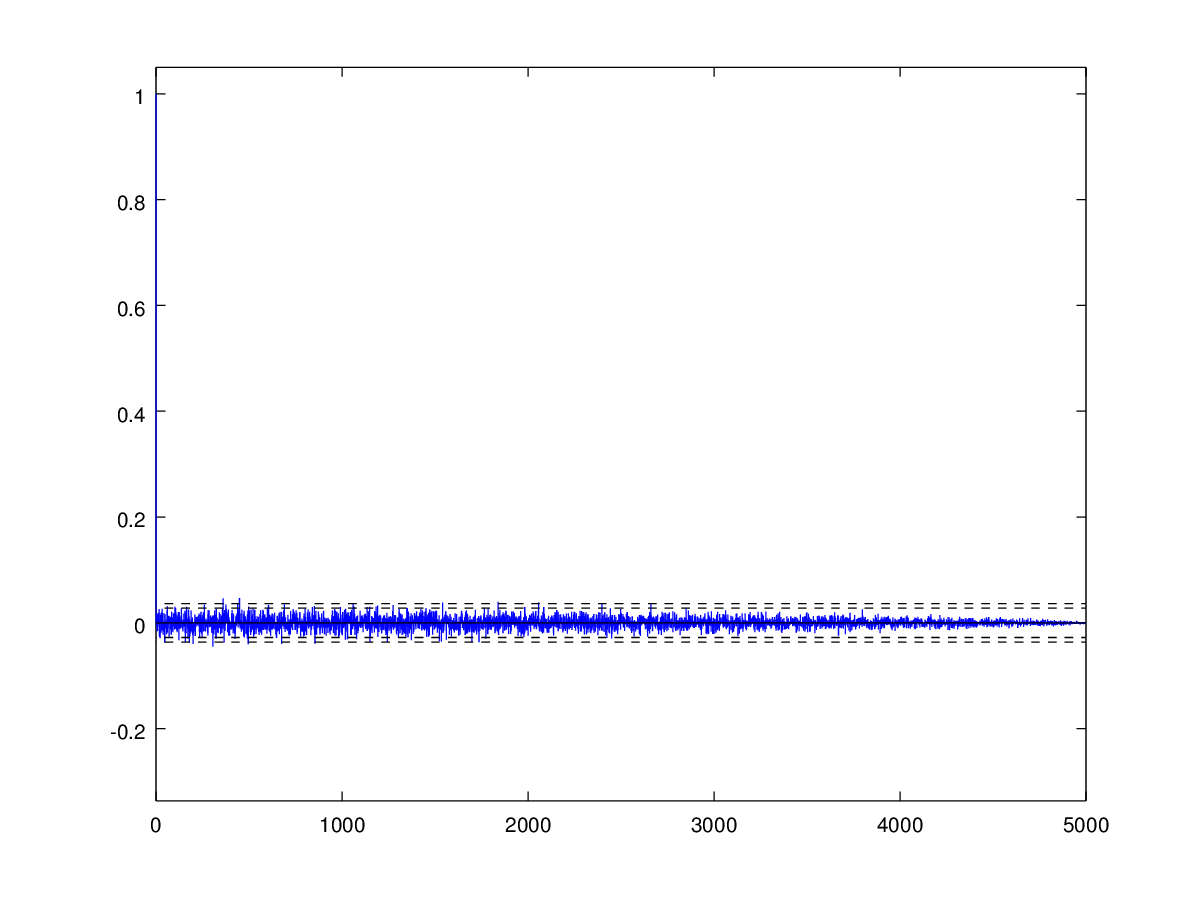
\includegraphics[width=\linewidth]{longAutocorr}
        \caption{Autocorrelation of a 5,000 iteration access pattern}
        \label{fig:longAutocorr}
    \end{subfigure}
    \caption{Two autocorrelation plots, with the autocorrelation coefficient on the y-axis and time lag on the x-axis. The dashed black lines represent confidence bands of 95\% and 99\%.}
    \label{fig:autocorr}
\end{figure}

The dashed black lines represent confidence bands of 95\% and 99\%, and in order to conclude that a sequence is random, we need almost all of the autocorrelation coefficients to lie within these bands. This is indeed the case, so ORAM has successfully taken a heavily non-random access pattern and turned it into a random one.

Runs testing attempts to detect non-random beheviour in a signal by counting the number of runs, sequences of values that are all above or below the median value. Too few runs in a sequence suggests a trend and too many runs suggests cyclic behaviour. For a large sample, we can approximate the distribution of runs using a normally distributed random variable, and compare this with the distribution that we measure. To generate the distribution, we take 1000 sample access patterns, each of length 180. We cut each pattern into 18 equally sized segments of size 10, take the mean of each segment, and count the number of runs in the sequence of means. There can be between 2 and 18 runs in each sequence, but we would expect 90\% of the sequences to have between 7 and 14 runs, the 0.05\% tail cut-offs for this distribution \cite{masliah2000stationarity}. \Cref{fig:runsTestPlot} plots this distribution, along with the tail cut-offs, and 92.2\% of samples fall within the bounds. Thus, we can conclude that the samples were generated from a random process.

\begin{figure}
    \centering
    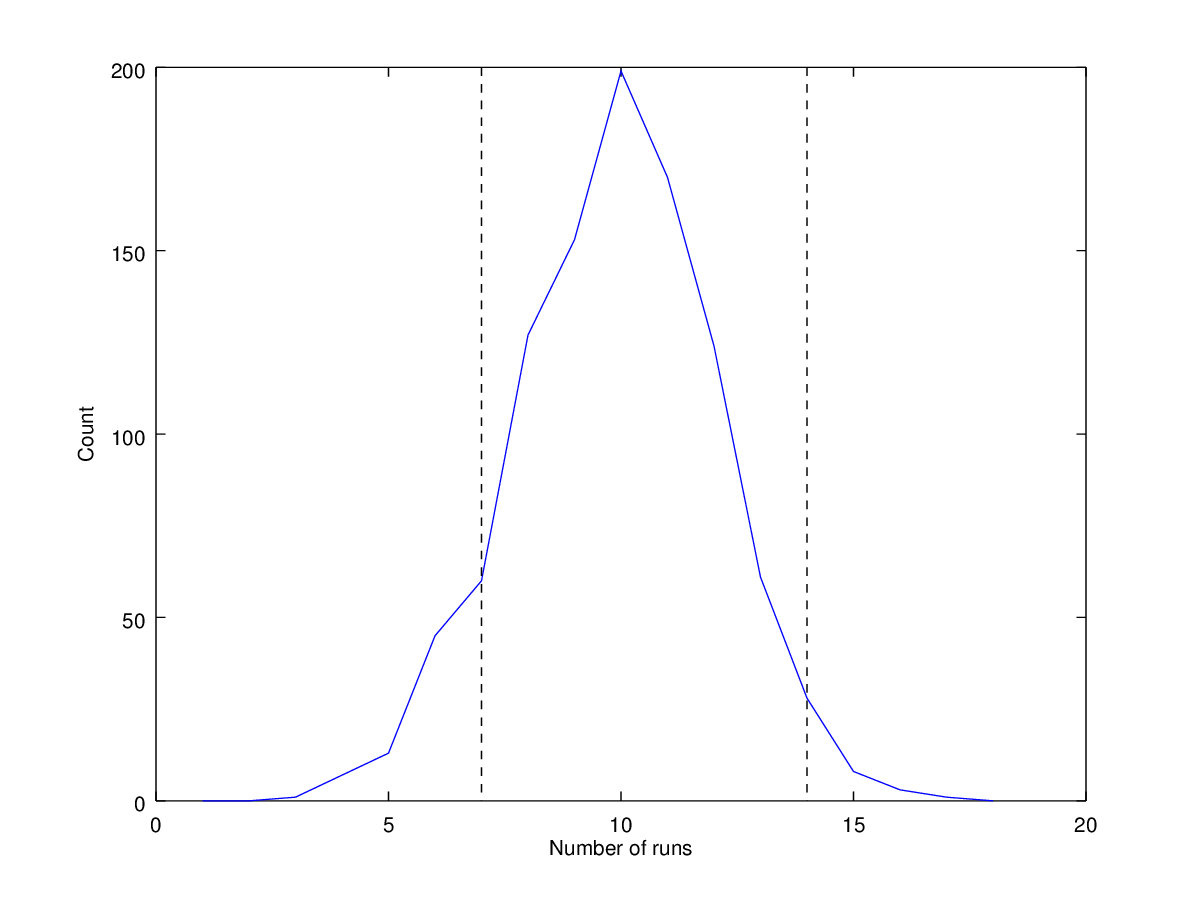
\includegraphics[width=.8\linewidth]{runsTestPlot}
    \caption{The distribution of the number of runs in 1000 access patterns of length 180. The dashed black lines represent 0.05\% tail cut-offs, and 92.2\% of values fall within these bounds.}
    \label{fig:runsTestPlot}
\end{figure}

\chapter{Conclusions}

\section{Results}

I successfully implemented the Path ORAM protocol and showed that my implementation agreed with the theoretical overhead of $O(\log N)$ and that it is a statistically secure implementation.

\section{Lessons Learnt}

This project has taught me many important lessons. The one that has had the most impact is time management. I got stuck into the project straight away and did as much work on it as I could during the Michaelmas term and vacation, which meant that hiccoughs later down the line had a large buffer and didn't cause severe consequences. Related to this I learnt that predicting the time that each part of a project will take is very difficult and it is therefore important to be both conservative and realistic about the number of things that will go wrong. I learnt the importance of sharing your work with others through contribution to the Mirage community and being invited to talk about the project at Microsoft Research Cambridge. I would like to thank Markulf Kohlweiss from Microsoft Research for giving his advice on the project and giving me the opportunity to present my finidings. Finally, I learnt that you should seek advice as soon as there are signs of trouble, rather than waiting for a scheduled meeting to bring something up. The advice of experienced supervisors can turn the seemingly catastrophic into a minor disruption.

\section{Future Work}

There is still much work to be done in the field of ORAM. One of the main drawbacks of current schemes is that the size of the ORAM must be determined in advance and the overhead associated with expanding it is enormous. I would like to investigate the possibility of creating a resizable version of my implementation, however this was unfortunately not in the scope of this project.

There are also many optimisations to be performed on this implementation. Along with many interesting optimisations mentioned in the literature, there is plenty of room for analysis and optimisation of this specific implementation using benchmarking to identify code hot-spots.

I would also like to perform further analysis to get a deeper understanding of this implementation. I would like to perform further experiments on the initialisation stage of ORAM to understand how the size of the stash changes during this period. I would also like to spend more time adjusting various parameters, including block size and bucket size, attempting to find an optimal set of values for them.

%%%%%%%%%%%%%%%%%%%%%%%%%%%%%%%%%%%%%%%%%%%%%%%%%%%%%%%%%%%%%%%%%%%%%
% the bibliography
\addcontentsline{toc}{chapter}{Bibliography}
\bibliography{refs}

%%%%%%%%%%%%%%%%%%%%%%%%%%%%%%%%%%%%%%%%%%%%%%%%%%%%%%%%%%%%%%%%%%%%%
% the appendices
\appendix

\chapter{Project Proposal}

% Note: this file can be compiled on its own, but is also included by
% diss.tex (using the docmute.sty package to ignore the preamble)
\documentclass[12pt,a4paper,twoside]{article}
\usepackage[pdfborder={0 0 0}]{hyperref}
\usepackage[margin=25mm]{geometry}
\usepackage{graphicx}
\begin{document}

\vfil

\centerline{\Large Computer Science Project Proposal}
\vspace{0.4in}
\centerline{\Large Encrypted Keyword Search Using}
\vspace{0.05in}
\centerline{\Large Path ORAM on MirageOS}
\vspace{0.4in}
\centerline{\large R. Horlick, Homerton College}
\vspace{0.3in}
\centerline{\large Originator: Dr N. Sultana}
\vspace{0.3in}
\centerline{\large 23 October 2015}

\vfil


\noindent
{\bf Project Supervisors:} Dr N. Sultana \& Dr R. M. Mortier
\vspace{0.2in}

\noindent
{\bf Director of Studies:} Dr B. Roman
\vspace{0.2in}
\noindent
 
\noindent
{\bf Project Overseers:} Dr M. G. Kuhn \& Prof P. M. Sewell


% Main document

\section*{Introduction and Description of the Work}

% Set the scene - change this so that it mentions that what we want is encrypted search

As the cost of large-scale cloud storage decreases and the rate of data production grows, more and more sensitive data is being stored in the cloud. We, of course, want to encrypt our data, to ward off prying eyes, but this comes at a cost. We can no longer selectively retrieve parts of the data at will. We need some method of searching over encrypted data to find the parts we are interested in.

% Set up the threat model for "honest but curious" adversary

So let us say that Alice has a set of documents that she wants to store on an untrusted server, run by Bob. We'll first assume that Bob is ``honest, but curious'', that is, he will attempt to gather all knowledge that he can without deviating from the protocol. Alice wants to store her documents encrypted, but also wants to search over them without Bob being able to learn either the keywords she is searching for, or the results of any query, the documents that contain the keyword. In order to enable efficient search over the documents, Alice stores an encrypted index on the server along with the documents.

There are a number of schemes in the literature that use symmetric encryption techniques to build a searchable encryption scheme. They rely on the use of a trapdoor generating function, that allows Bob to search over the encrypted index and respond to Alice with the matching line from the encrypted index. Then Alice requests the relevant documents from Bob. Bob has a complete view of the communications channel, but does not have access to the trapdoor generating function. He simply sees a query in the form of trapdoor and then a number of requests for specific documents.

The problem is that these all leak the access pattern, so Bob knows which documents matched any query, even if he doesn't know what they matched. It turns out that this pattern of access can leak large amounts of information. In a study \cite{islam2012access} on an encrypted email repository, up to 80\% of plaintext search queries could be inferred from the access pattern alone! So clearly this a leak worth plugging, but how can we do it? 

% Describe ORAM and mention Path ORAM

One solution to our problem is to use Oblivious Random Access Memory (ORAM), a cryptographic primitive that hides data access patterns. In our case, we move the searching and object retrieval functionality back to the client. That is, we turn Bob's server into a block device and we attempt to maintain the property that any two sequences of accesses of the form $(operation,address,data)$, that are the same length, have computationally indistinguishable physical access patterns. Bob should have no way of learning what $address$ we are really accessing, and therefore will never know which documents matched a given search query. 

A trivial ORAM algorithm operates by scanning over the whole ORAM and reading/updating only the relevant block, but this has $O(N)$ bandwidth cost, where $N$ is the number of blocks, which is highly impractical for large-scale storage. Luckily, much better algorithms have been proposed. We choose to focus on Path ORAM \cite{stefanov2013path}, because it has only $O(\log N)$ bandwidth cost in the worst case if $B = \Omega(\log^2 N)$, as well as being incredibly simple conceptually.

% Extend the threat model to incorporate malicious adversary and describe integrity protection techniques

Now let's assume that Bob has become malicious, and is modifying our encrypted data. In order to combat this, we can provide integrity verification by treating the ORAM as a Merkle tree, but with data in every node. The details of this scheme are outlined below after Path ORAM has been described further.

So the project is a searchable encrypted object store, with integrity verification. It will provide a simple, name-value pair API, that allows more complex filesystems to be built on top of it. A block diagram of the system is shown in Figure \ref{miragestack}.

%\begin{figure}
%\setlength{\unitlength}{0.75mm}
%\begin{center}
%\begin{picture}(170,70)
%\put(50,60){\framebox(50,10){Object Store}}
%
%\put(100,65){\vector(1,0){20}}
%\put(120,65){\vector(-1,0){20}}
%
%\put(120,60){\framebox(50,10){Indexed Search}}
%
%\multiput(44,55)(4,0){32}{\line(1,0){2}}
%\put(0,54){BLOCK Interface}
%\put(75,60){\vector(0,-1){10}}
%\put(75,50){\vector(0,1){10}}
%
%\put(145,45){\vector(0,1){15}}
%\put(145,45){\vector(-1,0){45}}
%
%\put(50,40){\framebox(50,10){ORAM}}
%
%\multiput(44,35)(4,0){32}{\line(1,0){2}}
%\put(0,34){BLOCK Interface}
%\put(75,40){\vector(0,-1){10}}
%\put(75,30){\vector(0,1){10}}
%
%\put(50,20){\framebox(50,10){Encryption}}
%
%\multiput(44,15)(4,0){32}{\line(1,0){2}}
%\put(0,14){BLOCK Interface}
%\put(75,20){\vector(0,-1){10}}
%\put(75,10){\vector(0,1){10}}
%
%\put(50,0){\framebox(50,10){BLOCK}}
%
%\end{picture}
%\end{center}
%\caption{The Application Stack: We can use any underlying BLOCK implementation and we can add/remove ORAM, Encryption or Search modules as we please}
%\label{miragestack}
%\end{figure}

\setlength{\unitlength}{0.75mm}
\begin{figure}[b]
\begin{center}
\begin{picture}(170,70)
\put(50,60){\framebox(50,10){File System}}

\put(100,65){\vector(1,0){20}}
\put(120,65){\vector(-1,0){20}}

\put(120,60){\framebox(50,10){Indexed Search}}

\multiput(44,55)(4,0){32}{\line(1,0){2}}
\put(0,54){BLOCK Interface}
\put(75,60){\vector(0,-1){10}}
\put(75,50){\vector(0,1){10}}

\put(145,45){\vector(0,1){15}}
\put(145,45){\vector(-1,0){45}}

\put(50,40){\framebox(50,10){ORAM}}

\multiput(44,35)(4,0){32}{\line(1,0){2}}
\put(0,34){BLOCK Interface}
\put(75,40){\vector(0,-1){10}}
\put(75,30){\vector(0,1){10}}

\put(50,20){\framebox(50,10){Encryption}}

\multiput(44,15)(4,0){32}{\line(1,0){2}}
\put(0,14){BLOCK Interface}
\put(75,20){\vector(0,-1){10}}
\put(75,10){\vector(0,1){10}}

\put(50,0){\framebox(50,10){BLOCK}}

\end{picture}
\end{center}
\caption{The application stack: ORAM satisfies MirageOS's \texttt{BLOCK} interace and any underlying \texttt{BLOCK} implementation can be used}
\label{miragestack}
\end{figure}

\section*{Starting Point}

% Explain Mirage (further explanation of Unikernel OS required) and justify its use

MirageOS is a framework, that pulls together a number of libraries and syntax extensions, to provide a lightweight unikernel operating system, that is designed to run on the Xen hypervisor. A unikernel operating system is a single-address space machine image, customised to provide the minimum set of features to run an application. It provides a command line tool for generating the main file, that links together implementations of various parts of the system, and passes them to the unikernel. There are a number of module signatures that define the operation of devices, such as CONSOLE for consoles, ETHIF for ethernet, and most importantly for us BLOCK, for block devices.

I have chosen to use Mirage for a number of reasons. Firstly, it is lightweight and designed to be run in the cloud, meaning that simple cloud services can be built on top of it that fully leverage the ORAM. Secondly, it is written in OCaml, meaning that I can take full advantage of static typing and a rich module system. 

This will allow me to write my implementation of ORAM and Encryption as a pair of functors that take an implementation of Mirage's BLOCK interface and create new BLOCK implementations, augmented with new features. This means that we can add and remove ORAM and Encryption as we like and the Object Store remains agnostic. This is shown in Figure \ref{miragestack}. It also means that we could use any underlying implementation of the BLOCK interface and that it would plug seamlessly into existing programs. There are currently two implementations of the BLOCK interface, one for Unix and one for Xen, and I would like to support both. This abstraction also allows for the use of cloud storage, implemented as a mapping between the BLOCK interface and a cloud provider's RESTful API.

Other OCaml libraries that will be of most use to me include nocrypto, which provides a wide variety of cryptographic tools, Jane Street's Core library, which standardises and optimises many of OCaml's core modules, and LWT, a lightweight cooperative threading library that is used throughout Mirage.

\section*{Substance and Structure of the Project}

\subsection*{Substance}

% Talk about the relative priorities of sections of the program

	% Main focus is ORAM, then we build object store on top of that, finally we implement the actual search module, but make it clear that, that is not the focus
	
	The main focus of this project is the implementation and evaluation of the Path ORAM protocol. Encrypted search is our target domain and as such will be an integral part of the project, but it is the performance and security properties that Path ORAM provides that we are really interested in.

% Describe Path ORAM protocol more clearly

The Path ORAM protocol has three main components: a binary tree, a stash and a position map. The binary tree is the main storage space. Every node in the tree is a bucket, which can contain up to $Z$ blocks. The tree has height $L$, where the tree of height 0 consists only of the root node, and the leaves are at level $L$. The stash is temporary client-side storage, consisting only of a set of blocks waiting to be put back into the tree. The position map associates, with each block ID, an integer between 0 and $2^L-1$. The invariant that the Path ORAM algorithm maintains is that if the position of a block $x$ is $p$, then $x$ is either in some bucket along the path from the root node to the $p^{th}$ leaf, or in the stash. On every access to the tree, a whole path is read into the stash, the accessed block is assigned a new random position and then as many blocks as possible are written back into the same path. The assignment to a random position means that, in any two access to the same block, the paths that are read are statistically independent.

% Describe recursive path oram protocol

We can extend the basic path ORAM algorithm with recursion. That is, calling the data ORAM $ORAM_0$, we store the position map of $ORAM_0$ in a smaller ORAM, $ORAM_1$, and the position map for this in an even smaller ORAM, $ORAM_2$. We can do this until we have a sufficiently small position map on the client. Supposing that we store $\chi$ leaf addresses in each PosMap ORAM, the position for a data block with address $a_0$ is at $a_1 = a_0 / \chi$ in $ORAM_1$, and in general $a_n = a_0 / \chi^n$ for the address in $ORAM_n$. 

% Mention that we want to be able to disconnect from the block device, so we'll need to be able to store the client state on the ORAM as well

There is actually an issue with using Path ORAM in the context of MirageOS and cloud storage. If the Mirage instance crashes, then we lose the client-side state. With no position map, the ORAM becomes useless. To remedy this, we would have to read the entire contents out in one go and then reinsert it, resulting in a large overhead. There are two solutions to this problem: store the client-side state in persistent storage on the client, or upload the state to the server after every access. The second option is preferable, because it separates the ORAM implementation from the client machine. The client-side state is actually $O(\log N)$, so we should be able to store it on the server without increasing our complexity bounds. 

% Talk about adding integrity verification of the ORAM

As mentioned above, we can add integrity verification to Path ORAM by treating it as a Merkle tree. Each node will store a hash of the form $H = (b_1||\cdots||b_n||h_1||h_2)$, where $b_n$ is the $n^{th}$ block stored in the node, and $h_1$ and $h_2$ are the hashes of the left and right children. We always read and write the whole path at a time, so for the read or write of any single node we only have to read or write two hashes. For instance, on write, we calculate the hash of the leaf node, which is then available for calculating the next level hash. So we only have to read the hash of the sibling of the leaf. This pattern is the same all the way up to the root of the tree.

% Discuss the search mechanism

In order to perform searches over our data, we will store along with it an encrypted inverted index. This is a data structure that, for any keyword, list the documents that contain it. The search module will build the index from the object store and then store the index using the object store. It will provide a search function that, given a keyword, will perform a simple scan over the inverted index and return the identifiers of documents that match it.

% Discuss evaluation techniques

\subsection*{Evaluation}

We need to test for functionality. Does the ORAM successfully write data and read it back out? Does the search function return documents correctly? This will consist of fairly trivial tests, writing objects to and from the block device and searching over them. A range of different types of documents will be used, including randomly (pre-)generated ones and entirely non-random ones, from sources such as Project Gutenberg.

We then want to evaluate performance. What is the overhead when we add the ORAM functor? How do recursion and statelessness further affect this? Does this correspond to the theoretical values from the literature? This will use tests similar to the above, but specifically focusing on time and space efficiency. Using the plain Object Store as a baseline, I will add in encryption and ORAM, separately and in combination to try and isolate the effects of each individual module. 

Finally we want to test the security properties of the project. Is there any statistical correlation between access patterns? Do we provide adequate integrity verification? What, if anything, can be inferred about the search queries? Apart from integrity verification, which we can test by simply corrupting the ORAM and making sure that this is detected, the security comes down to the statistical independence of access patterns. If we can show, using statistical methods, that there is no correlation between two sequences of accesses with identical length, then we have security for not just storage, but for search as well, because this is protected by ORAM's security.

\subsection*{Structure}

The project breaks down into the following sub-projects:

\begin{enumerate}

\item Familiarising myself with OCaml, MirageOS and related libraries

\item Implementing the basic Path ORAM functor and testing that it works in place of existing BLOCK device implementations

\item Implementing the Object Store, testing this and further testing ORAM using it

\item Adding recursion and statelessness to ORAM 

\item Implementing and testing the search module

\item Adding the encryption layer

\item Creation of a suite of tests and experiments to evaluate the performance and security properties of each individual component and of the system as a whole

\item Writing the dissertation

\end{enumerate}

\section*{Success Criteria for the Main Result}

\begin{enumerate}
	\item To demonstrate, through well chosen examples, that I have implemented a functionally correct Path ORAM functor with search capabilities
	\item To demonstrate, through well chosen examples, that the implementation has the expected security properties, i.e. keeps access patterns hidden
\end{enumerate}


\section*{Possible Extensions}

There are a number of ways that this project could be extended. By the nature of the modular design, we can perform optimisations at any layer of the system. There have been a large number of optimisations to Path ORAM proposed in the literature, so if I achieve the goals of my main project, including evaluation, ahead of schedule I will examine these and potentially implement some of them.

In particular for Path ORAM, recursion does add an overhead, but we can reduce this overhead by exploiting locality. Assuming that programs will access adjacent data blocks, we can cache PosMap blocks in a PosMap Lookaside Buffer, so that if all $\chi$ data blocks that are referenced in a PosMap block are accessed in turn we only need to do the recursion once. Doing this na\"ively, however, breaks security, because we are revealing information through the cache hit pattern. To avoid this we use Unified ORAM, which combines all of the recursive ORAMs into a single logical tree. We then use the address space to separate the levels of recursion, so addresses 1 to $N$ are for data blocks, $N + 1$ to $N + (N / \chi)$ for $ORAM_1$ and so on. Now all accesses occur in the same tree, and the security of Path ORAM keeps the cache miss pattern hidden.

Another optimisation compresses the PosMaps, reducing the number of levels of recursion required to achieve the desired client side storage, resulting in an asymptotic bandwidth complexity decrease for ORAM with small block size.

The last two optimisations were originally designed and tested in a secure processor setting \cite{ren2014unified}, so their application to the cloud storage setting is novel.

Another area that could be addressed is the limitation of Path ORAM (and other tree based ORAMs) to fixed-sized trees. We either need to know our storage requirements before setting up the ORAM, potentially wasting resources, or resize them in the na\"ive way as storage requirements increase. Resizability has been implemented for the ORAM construction of \emph{Shi et al.} \cite{shi2011oblivious} in \cite{moataz2015resizable}, but exploring the possibility of making Path ORAM resizable was left as an open research topic.

\section*{Timetable: Work plan and Milestones}

Planned starting date is 16/10/2015.

\begin{enumerate}

\item {\bf 16/10/15 -- 26/10/15} Familiarise myself with relevant Mirage libraries. Implement basic Path ORAM functor.

\item {\bf 27/10/15 -- 09/11/15} Implement basic test harness. Start implementation of object store.

\item {\bf 10/11/15 -- 23/11/15} Finish object store and use it to build more complex tests of the ORAM.

\item {\bf 24/11/15 -- 04/12/15} Add recursion and statelessness to the ORAM.

\item {\bf 05/12/15 -- 18/12/15} Write up implementation section of the dissertation for all parts completed so far.

\item {\bf 18/12/15 -- 31/12/15} Write the search module and design tests for it.

\item {\bf 01/01/16 -- 08/01/16} Write implementation section for the search module.

\item {\bf 09/01/16 -- 29/01/16} Evaluate the project in its current state, achieving an acceptably complete project. Write the progress report.

\item {\bf 30/01/16 -- 08/02/16} Write up the evaluation of the project so far.

\item {\bf 09/02/16 -- 21/02/16} Incorporate encryption model and perform further evaluation using this.

\item {\bf 22/02/16 -- 06/03/16} Submit first draft to supervisors for feedback and modify based on feedback.

\item {\bf 07/03/16 -- 11/03/16} Perform further evaluation and refinement as necessary

\item {\bf 12/03/16 -- 25/03/16} Write final draft of dissertation and then leave it until submission time, in order to focus on revision.

\item {\bf 01/05/16 -- 13/05/16} Reread and make any final edits and then submit.

\end{enumerate}

\section*{Resources Required}

\begin{itemize}

	\item My own laptop for implementation and testing

	\item My own external hard disk for backups

	\item GitHub for version control and backup storage

	\item MirageOS libraries as a basis for the project

\end{itemize}

\end{document}


\end{document}
